\documentclass[11pt, a4paper]{article}
\usepackage[margin=1.1in]{geometry}	% edit margins
\usepackage{amsmath}			% for math symbols
\usepackage{graphicx}			% including figures
\usepackage{grffile}			% for weird filenames with more dots
\usepackage{float}			% placing figures at specific location
\usepackage{amssymb}			% math symbols
\usepackage{color, soul}		% for highlighting
\usepackage{mathtools}			% for text over equals sign
% \usepackage{./use/mcode}		% for including code


\begin{document}

\title{Final Project: Orbit Determination\\ ASEN 5044 Statistical Estimation}
\author{Keith Covington\\Connor Ott}
\date{December 18, 2019}
\maketitle



%%%%%%%%%%%%%%%%%%%%%%%%%%%%%%%%% INTRODUCTION  %%%%%%%%%%%%%%%%%%%%%%%%%%%%%%%%%
\section*{Introduction}
In order to keep track of Earth-orbiting objects, a typical observation scheme includes ground stations which measure range and range-rate to a passing satellite. 
These measurements, when combined with the known locations of the stations, allows for precises estimates of a satellites orbit state. 
In addition to an orbit estimate, it's usually useful to quantify the uncertainty in the estimate. 
This quantity is a based on the uncertainty in the motion of the satellite in orbit, and the uncertainty in the incoming measurements. 
Neither of these uncertainties are necessarily known.
In order to accurately predict an estimate uncertainty, both of these uncertainties must be balanced with each other. 
This is frequently carried out with predictor-corrector estimation algorithm such as the Linearized Kalman Filter (LKF) or Extended Kalman Filter (EKF.)

In this report, we explore the performance of the LKF and EKF on nonlinear systems with dynamic uncertainty (process noise) and measurement uncertainty (measurement nose.) 
In developing these algorithms, we assume the process and measurement noise are unknown.
We then iterate on different process noise and measurement noise covariance matrices and evaluate the algorithms using Normalized Estimation Error Squared (NEES) and Normalized Innovation Squared (NIS) tests until suitable values for uncertainty are found. 

\section{Basic System Analysis}
\label{sec: Part I}

To study the LKF and EKF, we establish an estimation problem in the context of orbit determination. 
The following section describes the continuous-time system used in this study for dynamics and measurements.
The state of an orbiting object is described by its position and velocity in a 2D plane with the vector $x = [X, \dot{X}, Y, \dot{Y}]^T = [x_1, x_2, x_3, x_4]$.

The full CT, non-linear equations of motion for this system are shown below:


Equations of motion:
$$
f(x) = \dot{x} = 
\left[\begin{matrix}
x_2 \\
-\frac{\mu x_1}{(x_1^2 + x_3^2)^{3/2}} + u_1 + \tilde{w}_1 \\
x_4 \\
-\frac{\mu x_3}{(x_1^2 + x_3^2)^{3/2}} + u_2 + \tilde{w}_2
\end{matrix}\right]
$$
\indent Measurement function:
$$
h(x) = y = 
\left[\begin{matrix}
\sqrt{(x_1 - x^{(i)}_s)^2 + (x_3 - y^{(i)}_s)^2}\\
\frac{\left[x_1 - x^{(i)}_s\right]\left[x_2 - \dot{x}^{(i)}_s\right] + \left[x_3 - y^{(i)}_s\right]\left[x_4 - \dot{y}^{(i)}_s\right]}{h_1} \\
\tan^{-1}\big(\frac{x_3 - y^{(i)}_s}{x_1 - x^{(i)}_s} \big)\\
\end{matrix}\right]
$$

In the equation $h(x) = y$, terms a superscript (i) denotes the position or velocity of one of 12 ground stations currently viewing the spacecraft. 
These stations' position and velocity is assumed to be known completely.


\subsection{CT Model Jacobians}

$$
\tilde{A} = \frac{\partial f}{\partial x} \biggr\rvert_{nom} = 
\left[\begin{matrix}0 & 1 & 0 & 0\\\frac{3\mu x_{1}^{2}}{\left(x_{1}^{2} + x_{3}^{2}\right)^{5/2}} - \frac{\mu}{\left(x_{1}^{2} + x_{3}^{2}\right)^{3/2}} & 0 & \frac{3\mu x_{1} x_{3}}{\left(x_{1}^{2} + x_{3}^{2}\right)^{5/2}} & 0\\0 & 0 & 0 & 1\\\frac{3\mu x_{1} x_{3}}{\left(x_{1}^{2} + x_{3}^{2}\right)^{5/2}} & 0 & \frac{3\mu x_{3}^{2}}{\left(x_{1}^{2} + x_{3}^{2}\right)^{5/2}} - \frac{\mu}{\left(x_{1}^{2} + x_{3}^{2}\right)^{3/2}} & 0\end{matrix}\right]
$$

$$
\tilde{B} = \frac{\partial f}{\partial u} \biggr\rvert_{nom} = 
\left[\begin{matrix}0 & 0\\1 & 0\\0 & 0\\0 & 1\end{matrix}\right]
$$

$$
\tilde{\Gamma} = \frac{\partial f}{\partial w} \biggr\rvert_{nom} = 
\left[\begin{matrix}0 & 0\\1 & 0\\0 & 0\\0 & 1\end{matrix}\right]
$$

$$
\tilde{H} = \frac{\partial h}{\partial x} \biggr\rvert_{nom} = 
\left[\begin{matrix}
\tilde{H}_{11} & \tilde{H}_{12} & \tilde{H}_{13} &  \tilde{H}_{14}\\
\tilde{H}_{21} & \tilde{H}_{22} & \tilde{H}_{23} &  \tilde{H}_{24}\\
\tilde{H}_{31} & \tilde{H}_{32} & \tilde{H}_{33} &  \tilde{H}_{34}
\end{matrix}\right]
$$

Where: 
\begin{align*}
\tilde{H}_{11} &= \frac{x_{1} - x_s}{\left(\left(x_{1} - x_s\right)^{2} + \left(x_{3} - y_s\right)^{2}\right)^{1/2}} \\
\tilde{H}_{12} &= 0 \\
\tilde{H}_{13} &= \frac{x_{3} - y_s}{\left(\left(x_{1} - x_s\right)^{2} + \left(x_{3} - y_s\right)^{2}\right)^{1/2}} \\
\tilde{H}_{14} &= 0 \\
\tilde{H}_{21} &= \frac{\left(x_s - x_{1}\right) \left(\left(x_{1} - x_s\right) \left(x_{2} - \dot{x}_s\right) + \left(x_{3} - y_s\right) \left(x_{4} - \dot{y}_s\right)\right)}{\left(\left(x_{1} - x_s\right)^{2} + \left(x_{3} - y_s\right)^{2}\right)^{3/2}} + \frac{x_{2} - \dot{x}_s}{\left(\left(x_{1} - x_s\right)^{2} + \left(x_{3} - y_s\right)^{2}\right)^{1/2}} \\
\tilde{H}_{22} &= \frac{x_{1} - x_s}{\left(\left(x_{1} - x_s\right)^{2} + \left(x_{3} - y_s\right)^{2}\right)^{1/2}} \\
\tilde{H}_{23} &= \frac{\left(- x_{3} + y_s\right) \left(\left(x_{1} - x_s\right) \left(x_{2} - \dot{x}_s\right) + \left(x_{3} - y_s\right) \left(x_{4} - \dot{y}_s\right)\right)}{\left(\left(x_{1} - x_s\right)^{2} + \left(x_{3} - y_s\right)^{2}\right)^{3/2}} + \frac{x_{4} - \dot{y}_s}{\left(\left(x_{1} - x_s\right)^{2} + \left(x_{3} - y_s\right)^{2}\right)^{1/2}} \\
\tilde{H}_{24} &= \frac{x_{3} - y_s}{\left(\left(x_{1} - x_s\right)^{2} + \left(x_{3} - y_s\right)^{2}\right)^{1/2}}\\
\tilde{H}_{31} &= \frac{y_s - x_{3}}{\left(x_{1} - x_s\right)^{2} + \left(x_{3} - y_s\right)^{2}} \\
\tilde{H}_{32} &= 0 \\
\tilde{H}_{33} &= \frac{x_{1} - x_s}{\left(x_{1} - x_s\right)^{2} + \left(x_{3} - y_s\right)^{2}} \\
\tilde{H}_{34} &= 0 \\
\end{align*}

\subsection{DT Linearized Model Matrices}
Below are the equations for the DT jacobians.
\begin{equation}
	\begin{aligned}
		\tilde{F} &= I + \Delta t \cdot \tilde{A} \\
		\tilde{G} &= \Delta t \cdot \tilde{B} \\
		\tilde{\Omega} &= \Delta t \cdot \tilde{\Gamma}
	\end{aligned}
\end{equation}


\subsection{Simulated Nonlinear vs. Linearized System}
Figure \ref{fig:nlvl_s} shows the difference between propagating a small initial perturbation using full nonlinear dynamics and DT state transition matrices. 
These were gathered by propagating two orbits, a nominal and initially perturbed orbit, with full nonlinear dynamics using an RK45 integration method.
The difference between these orbits is shown by the blue line in Figure \ref{fig:nlvl_s}. 
The initial perturbation (difference between the initial states of the nonlinear trajectories described above) was then propagated using the linearized DT jacobians evaluated on the nominal trajectory. 
The linear propagation of the perturbation is shown in red. 
The nonlinear and linear perturbations stay near each other for the first half of an orbit, but quickly grow apart.
This indicates that the linearized dynamics are only appropriate for short time spans while the perturbed orbit remains relatively close to the nominal orbit where the DT jacobians are evaluated. 

\begin{figure}[H]
	\centering
	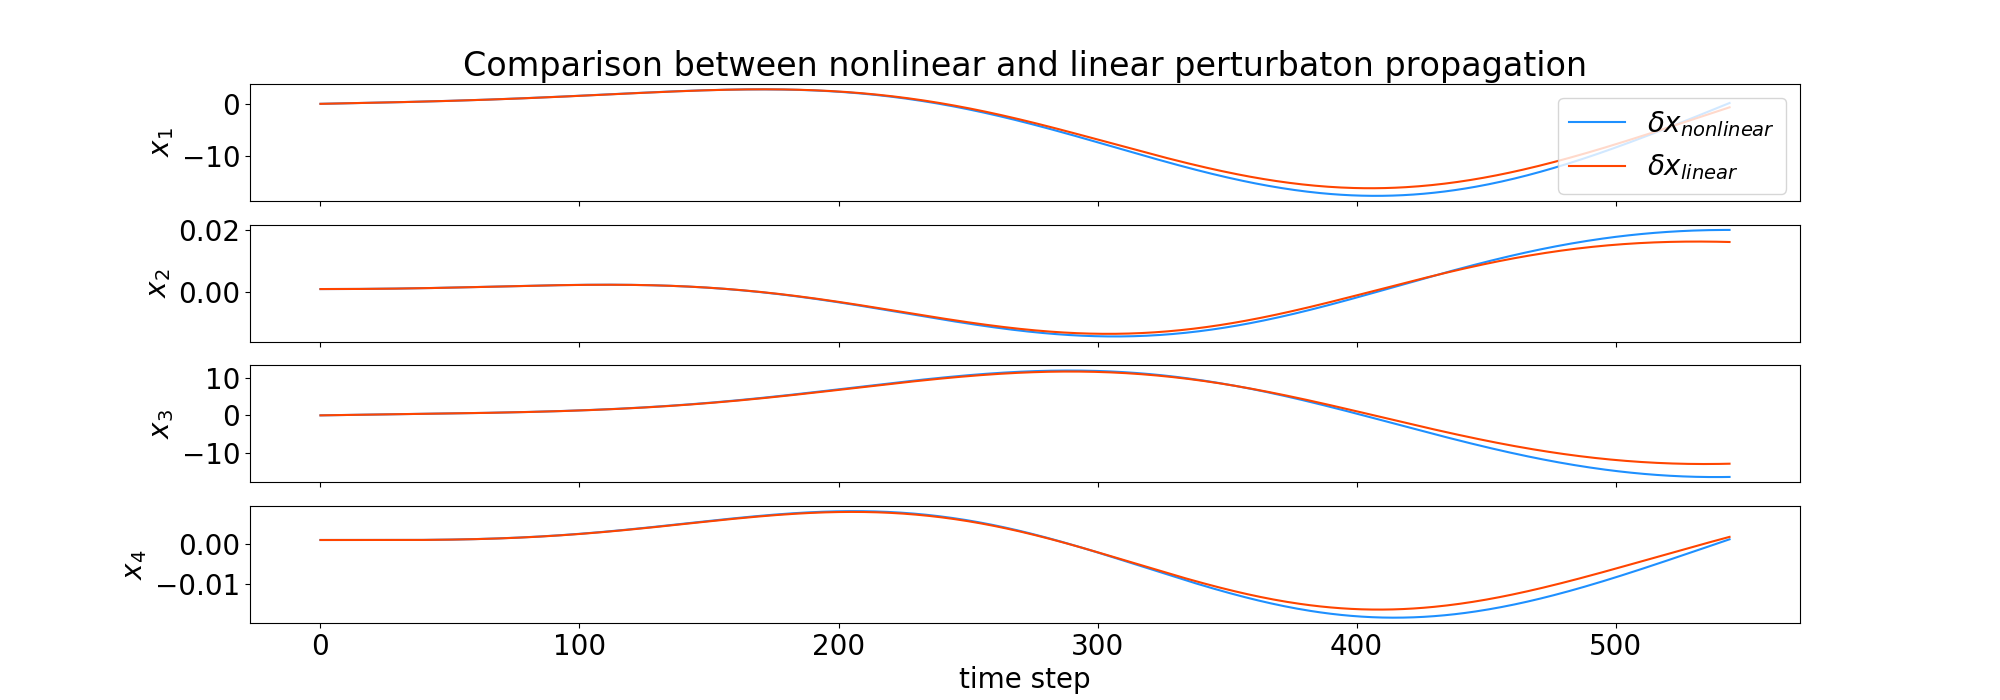
\includegraphics[width=\textwidth]{./Figures/nonlvl_state.png}
	\caption{Comparison between nonlinear and linear perturbation propagation.}
	\label{fig:nlvl_s}
\end{figure}

We draw similar conclusions about the validity of the linearized measurement function from Figure \ref{fig:nlvl_m}.
As the perturbed orbit drifts further and further from the nominal orbit, the linearized dynamics and measurement function are unable to closely match the nonlinear dynamics. 
 

\begin{figure}[H]
	\centering
	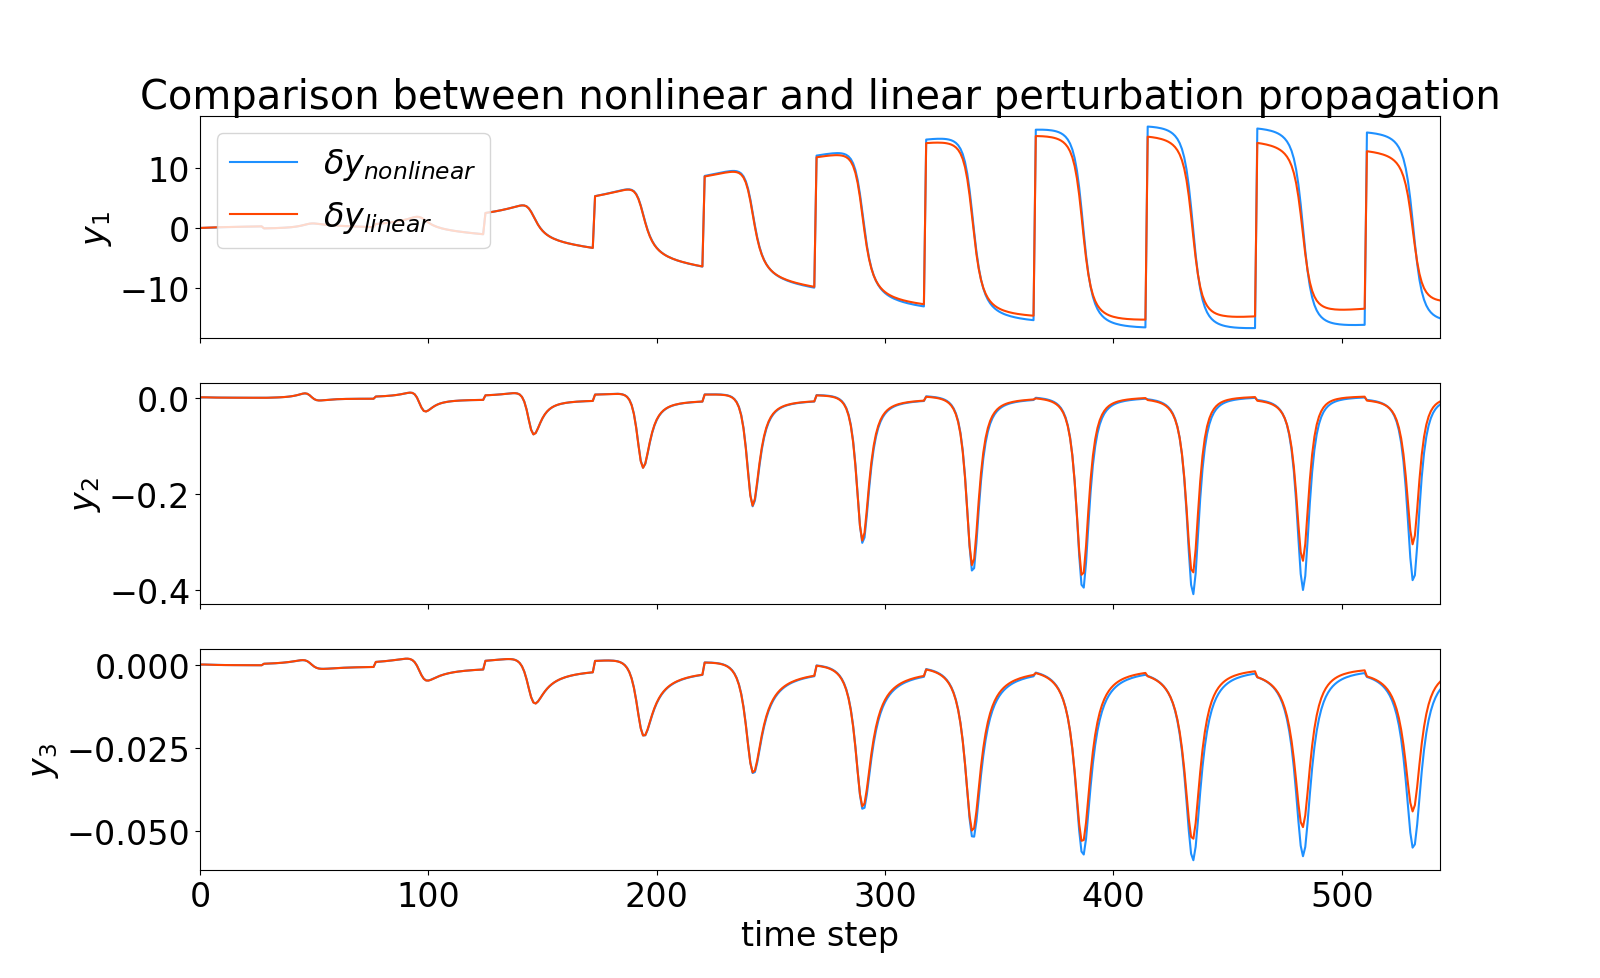
\includegraphics[width=\textwidth]{./Figures/nonlvl_meas.png}
	\caption{Comparison between nonlinear and linear perturbation propagation.}
	\label{fig:nlvl_m}
\end{figure}


\section{Nonlinear Filtering}
This section delves into the capabilities of the LKF and EKF in with respect to estimating nonlinear trajectories. 
We explore this through simulated orbits wherein truth states are generated with a deviation from the nominal initial conditions, and process noise (AWGN) added the dynamics of the system. 
The process noise is added to the spacecraft accelerations via a Zero Order Hold over each discrete time step in the integrator. 
The noisy, perturbed truth states are mapped to measurement space through the nonlinear measurement equation and measurement combined with white Gaussian.
Process and measurement noise are both sampled from $Q_{true}$ and $R_{true}$ given in the assignment data when generating truth trajectories.

Each truth trajectory is initially perturbed with the same $\delta x_0$ sampled from a chosen $P_0$. These are $P_0$ = diag([$10m^2, 1m^2/s^2, 10m^2, 1m^2/s^2$]) and $\delta x_0$ = [0.078 km, 0.022 km/s, -0.058 km, 0.031 km/s].
All filters begin with this initial estimate either as a deviation of full state, and all begin with this initial covariance. 


\subsection{The Linearized Kalman Filter}
\label{sec: LKF}
The LKF revolves around the concept of linearizing dynamics and measurement functions around a nominal trajectory at discrete time steps in the filter. 
This has its benefits in terms of simplicity and computational load, but suffers in terms of accuracy with relatively large deviations from the nominal trajectory. 

\subsubsection{LKF Typical Performance}
Figures \ref{fig:noisey_states} and \ref{fig:noisey_meas} show a typical noisy truth trajectory and accompanying noisey measurements as compared to the nominal, noiseless trajectory and measurements. 
We note here that the noise is largely drowned out by the effect of the initial perturbation. 
For Figure \ref{fig:noisey_meas}, both sets of measurements are generated as if they can see the same stations at each time step. 
Near the start of the simulation, this is mostly true, but the two trajectories quickly move apart and the difference in measurements becomes more jarring.

\begin{figure}[H]
	\centering
	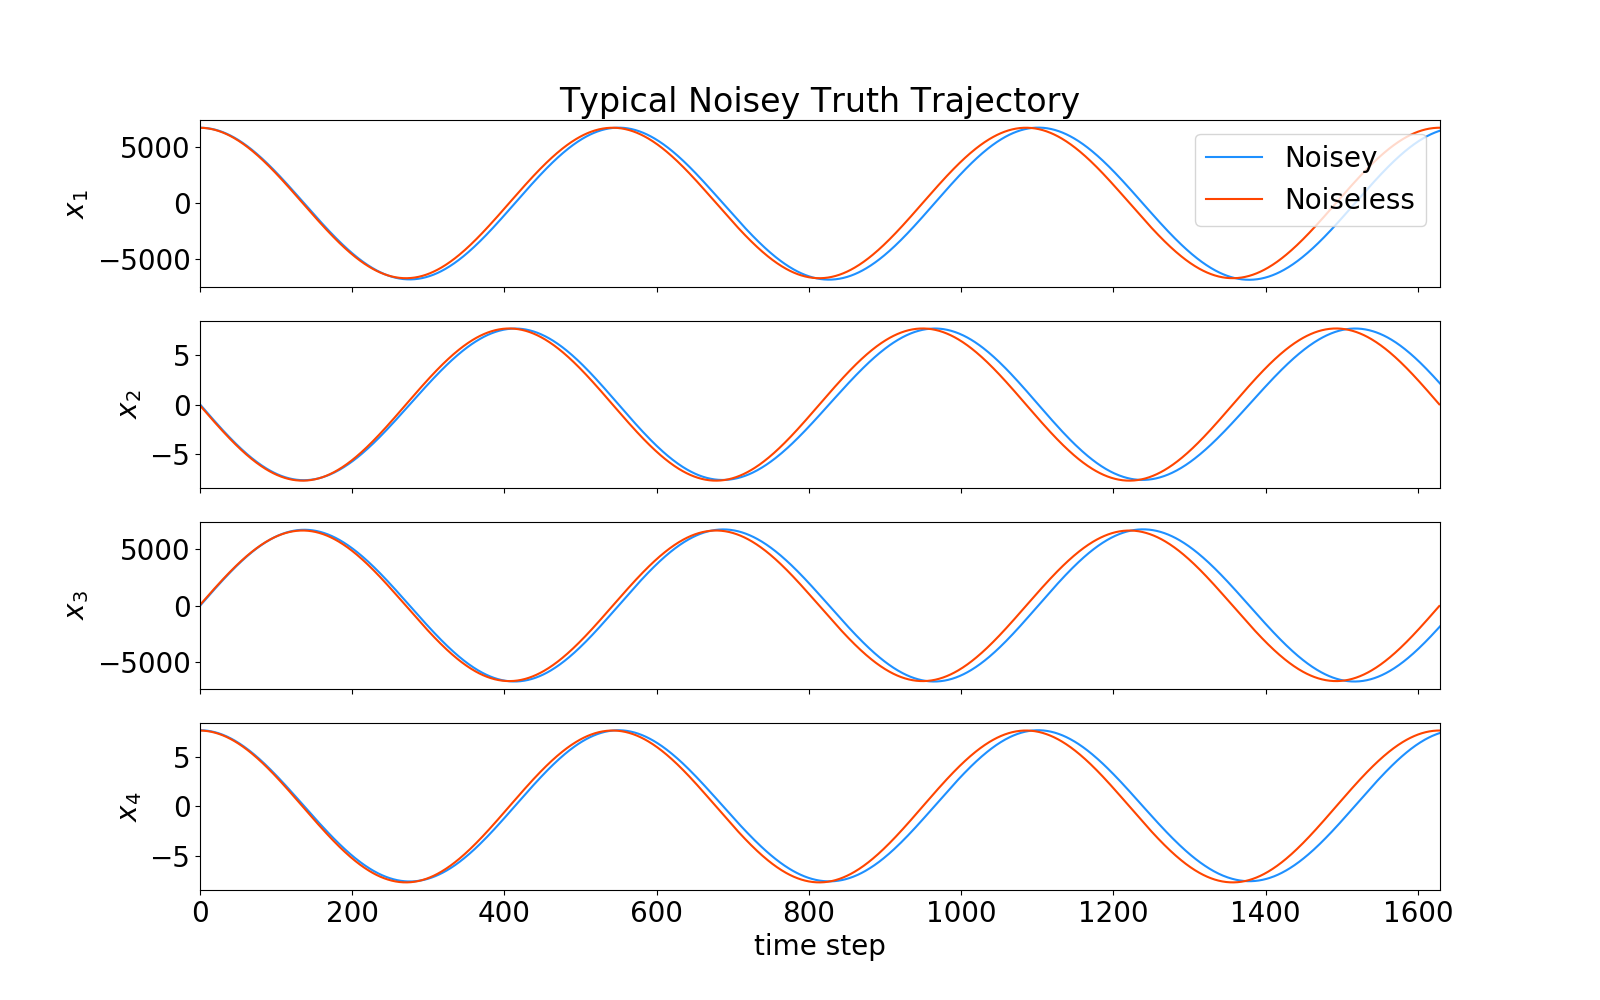
\includegraphics[width=\textwidth]{Figures/noisey_truth.png}
	\caption{Typical noisy trajectory as compared to the nominal, noiseless trajectory.}
	\label{fig:noisey_states}
\end{figure}

\begin{figure}[H]
	\centering
	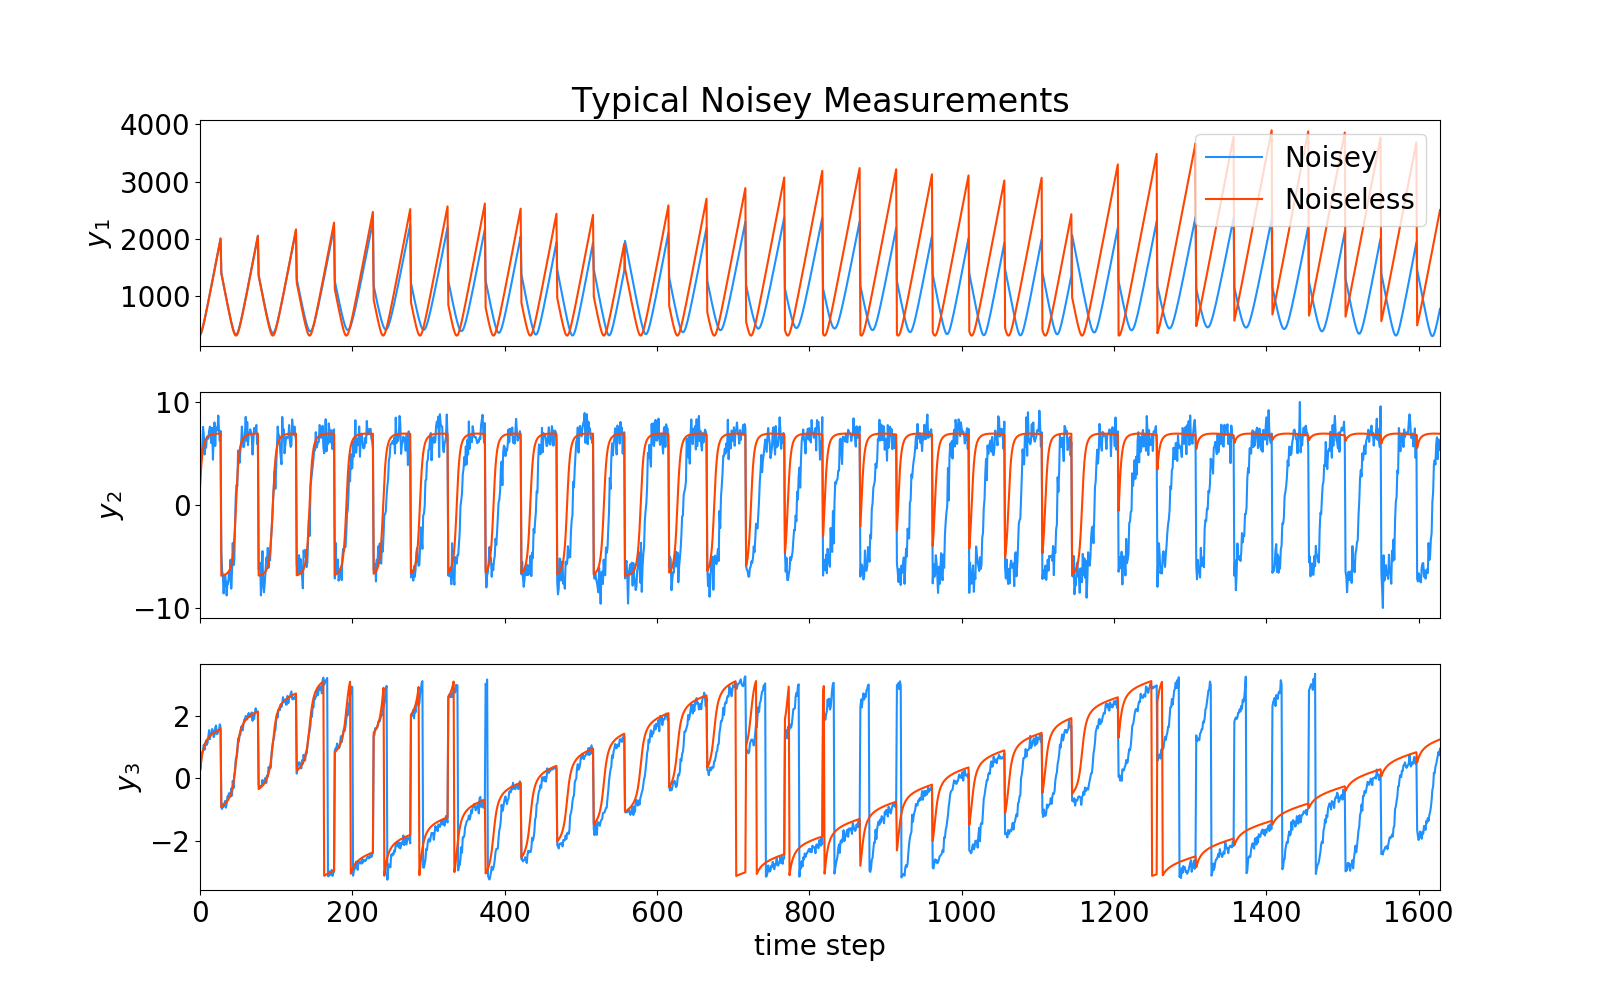
\includegraphics[width=\textwidth]{Figures/noisey_meas.png}
	\caption{Typical noisy measurements as compared to the nominal, noiseless measurements.}
	\label{fig:noisey_meas}
\end{figure}

Figure \ref{fig:lkf_est_zoom} shows the LKF estimate error and uncertainty bounds for the first 100 time steps (1e4 seconds) for a single simulation. 
The filter performs adequately for these first 100 time steps.
However, as time goes on, and the truth trajectory deviates further from the nominal, the LKF is unable to estimate an accurate trajectory.

Figure \ref{fig:lkf_est} shows the rapidly deteriorating estimate error in the LKF.  

\begin{figure}[H]
	\centering
	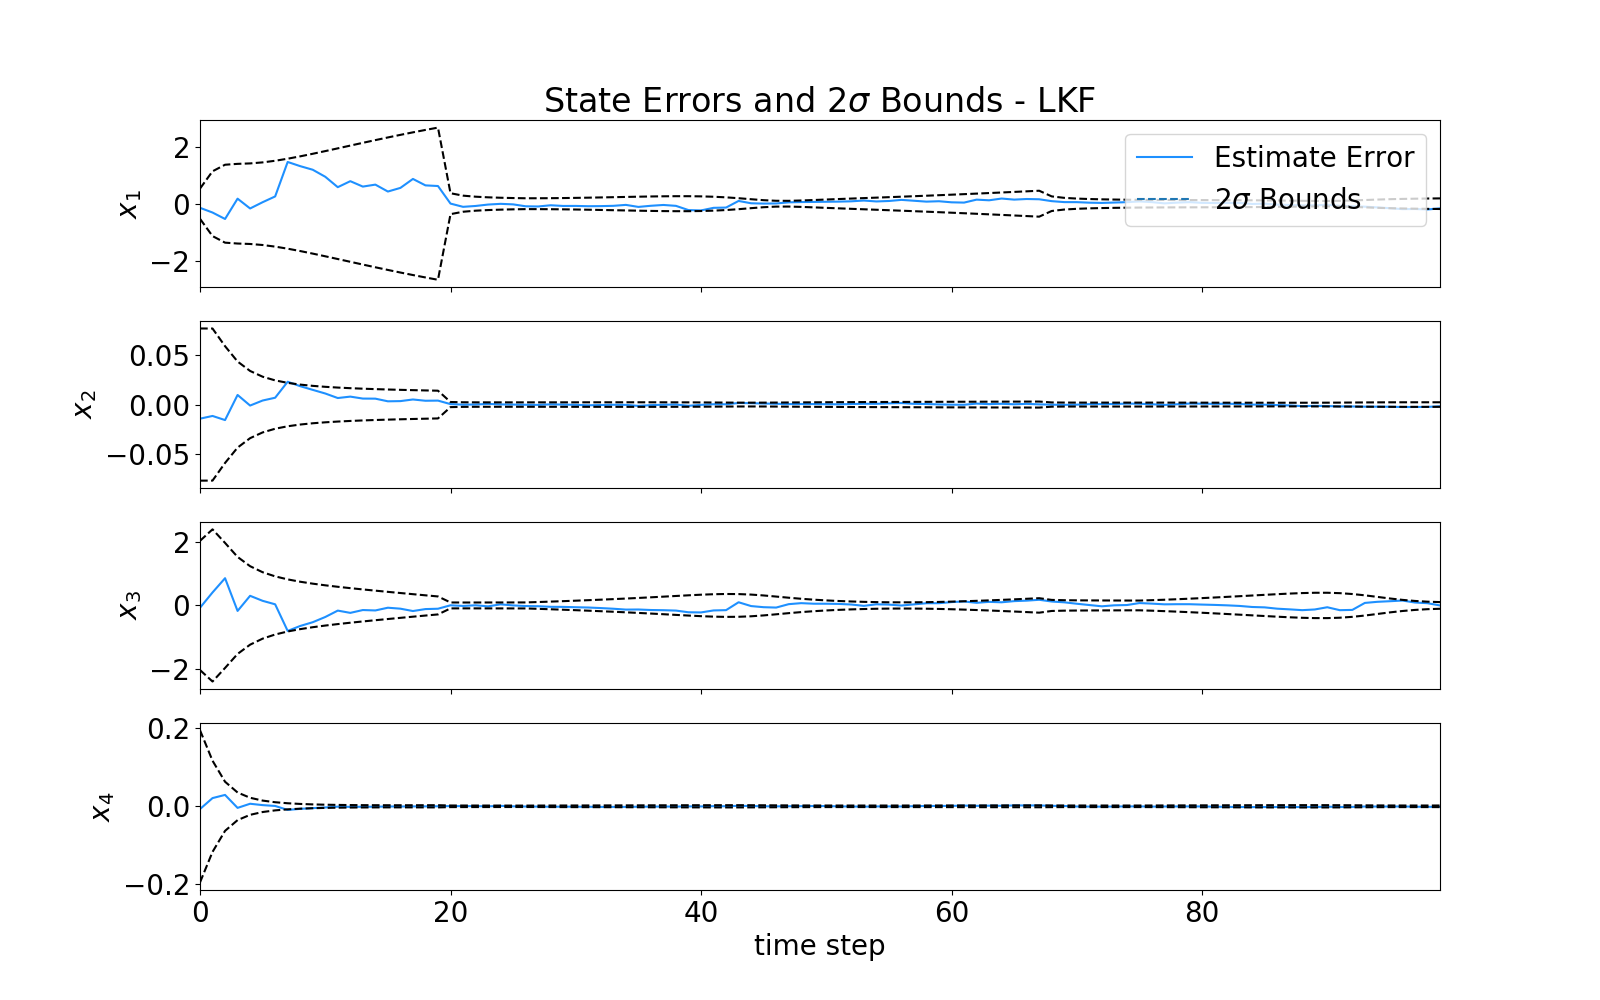
\includegraphics[width=\textwidth]{Figures/lkf_estimate_th_ZOOM.png}
	\caption{Typical LKF estimate for first 100 time steps (1e4 seconds or $\approx$1/5 of an orbit.)}
	\label{fig:lkf_est_zoom}
\end{figure}

\begin{figure}[H]
	\centering
	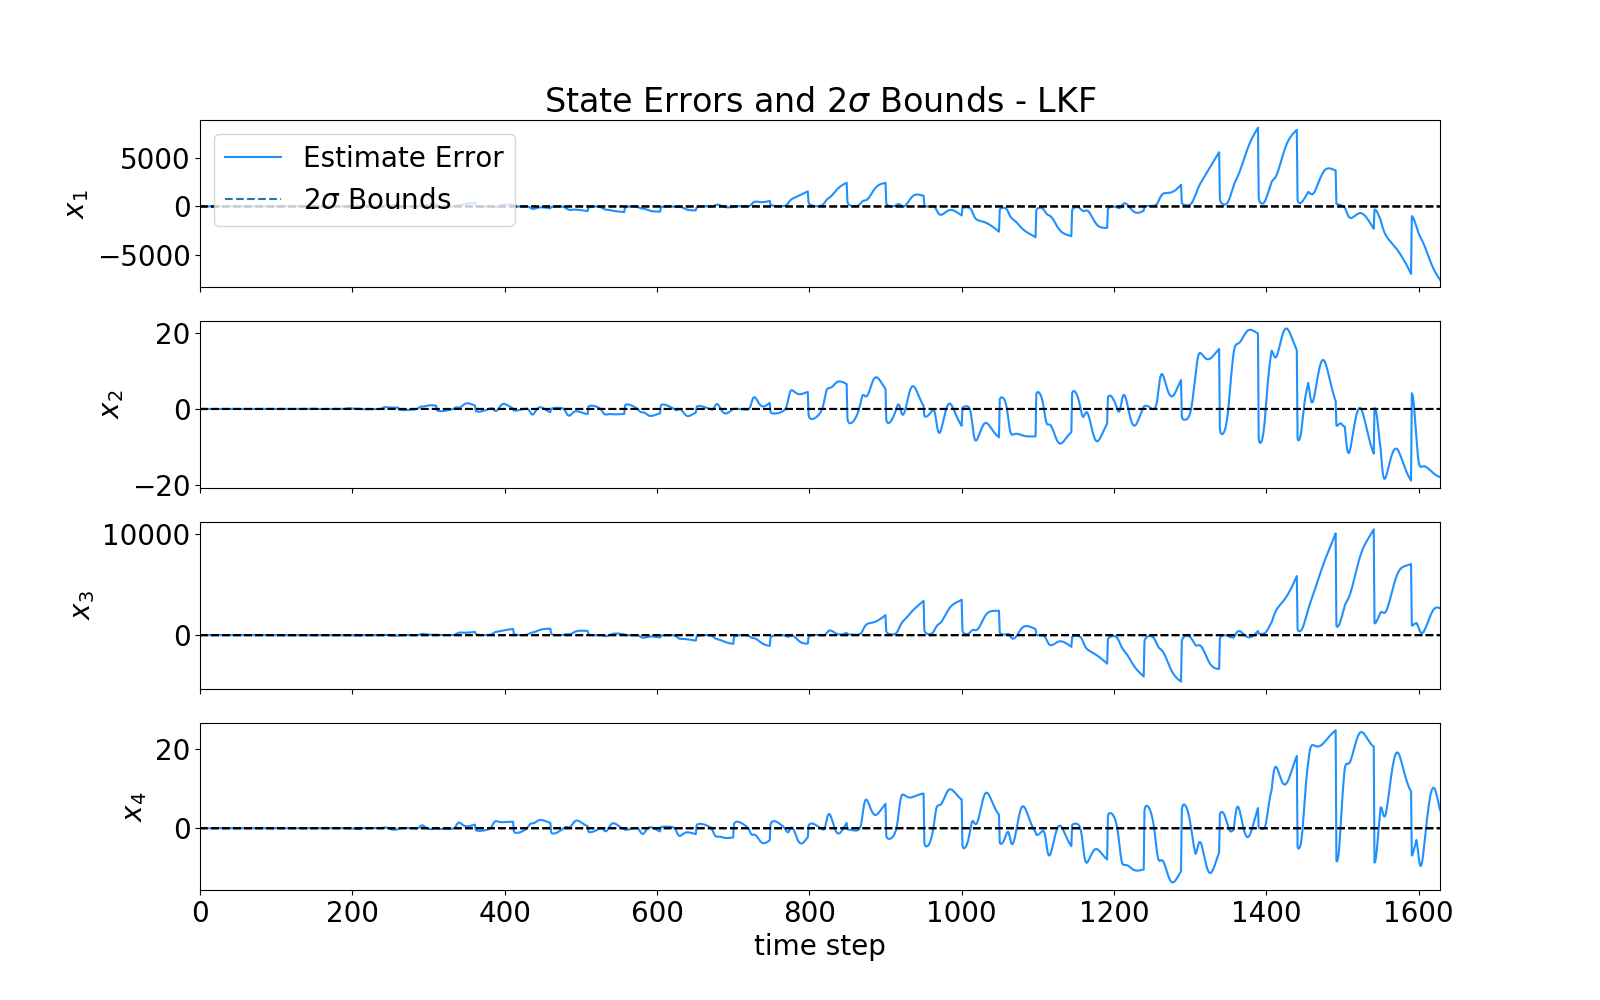
\includegraphics[width=\textwidth]{Figures/lkf_estimate_th.png}
	\caption{Typical LKF estimate for entire simulation.}
	\label{fig:lkf_est}
\end{figure}

\subsubsection{LKF NEES and NIS Tests}
The following are results of NEES and NIS chi-square tests for an implementation of the LKF. 
In the following figures, we plot NEES and NIS values from the filter at time k, averaged over N simulated trajectories. 
The equations for a given NEES and NIS equations at a time $k$ is given by Equations \ref{eq:NEES} and \ref{eq:NIS}, respectively.
\begin{equation}
	\epsilon_{x,k} = e^T_{x,k} (P^+_k)^{-1} e_{x,k},
	\quad \text{where} \quad
	e_{x,k} = x_k - \hat{x}^+_k
	\label{eq:NEES}
\end{equation}
\begin{equation}
	\epsilon_{y,k} = e^T_{y,k} (S_k)^{-1} e_{y,k},
	\quad \text{where} \quad
	e_{y,k} = y_k - \hat{y}^-_k
	\label{eq:NIS}
\end{equation}
At each time step, the NEES and NIS values are expected to fall into 4 (NEES) or 3 (NIS) degree of freedom $\mathcal{X}^2$ distributions. 
As such, we expect values to fall within some range of the expectation of these distributions. 
For this study, we've chosen 95\% confidence bounds, which are denoted with the dotted black lines. 
The filter was tuned by adjusting the filter's knowledge of process noise in the system until the simulations reliably generated NEES and NIS results within the confidence bounds at least 95\% of the time. 
Note that in the NEES/NIS test below, only a time span of $k\ \epsilon\ [0, 150]$ is shown due to the LKF's poor performance further into the orbit. 
Additionally, note that $N$ was chosen to be 10 for the purpose of minimizing computational time, while still conveying the information gathered from these tests. In deciding N, it was found that increasing N past 10 did no provide substantial insight to filter performance for the increase in computational time. 

In this first iteration of the tuning process, the Kalman filter was initialized with an internal (guessed) process noise of $Q_{KF} = 10^{-6} \cdot I_{2 x 2}$. 
The results of this test can be seen in Figure \ref{fig:neesnis_lkf_Qbig}. 
In both tests---but especially the NEES---the values are biased below the lower confidence bound. 
This low bias led to the conclusion that the guessed $Q_{KF}$ is too large and can be lowered for better filter performance. 
\begin{figure}[H]
	\centering
	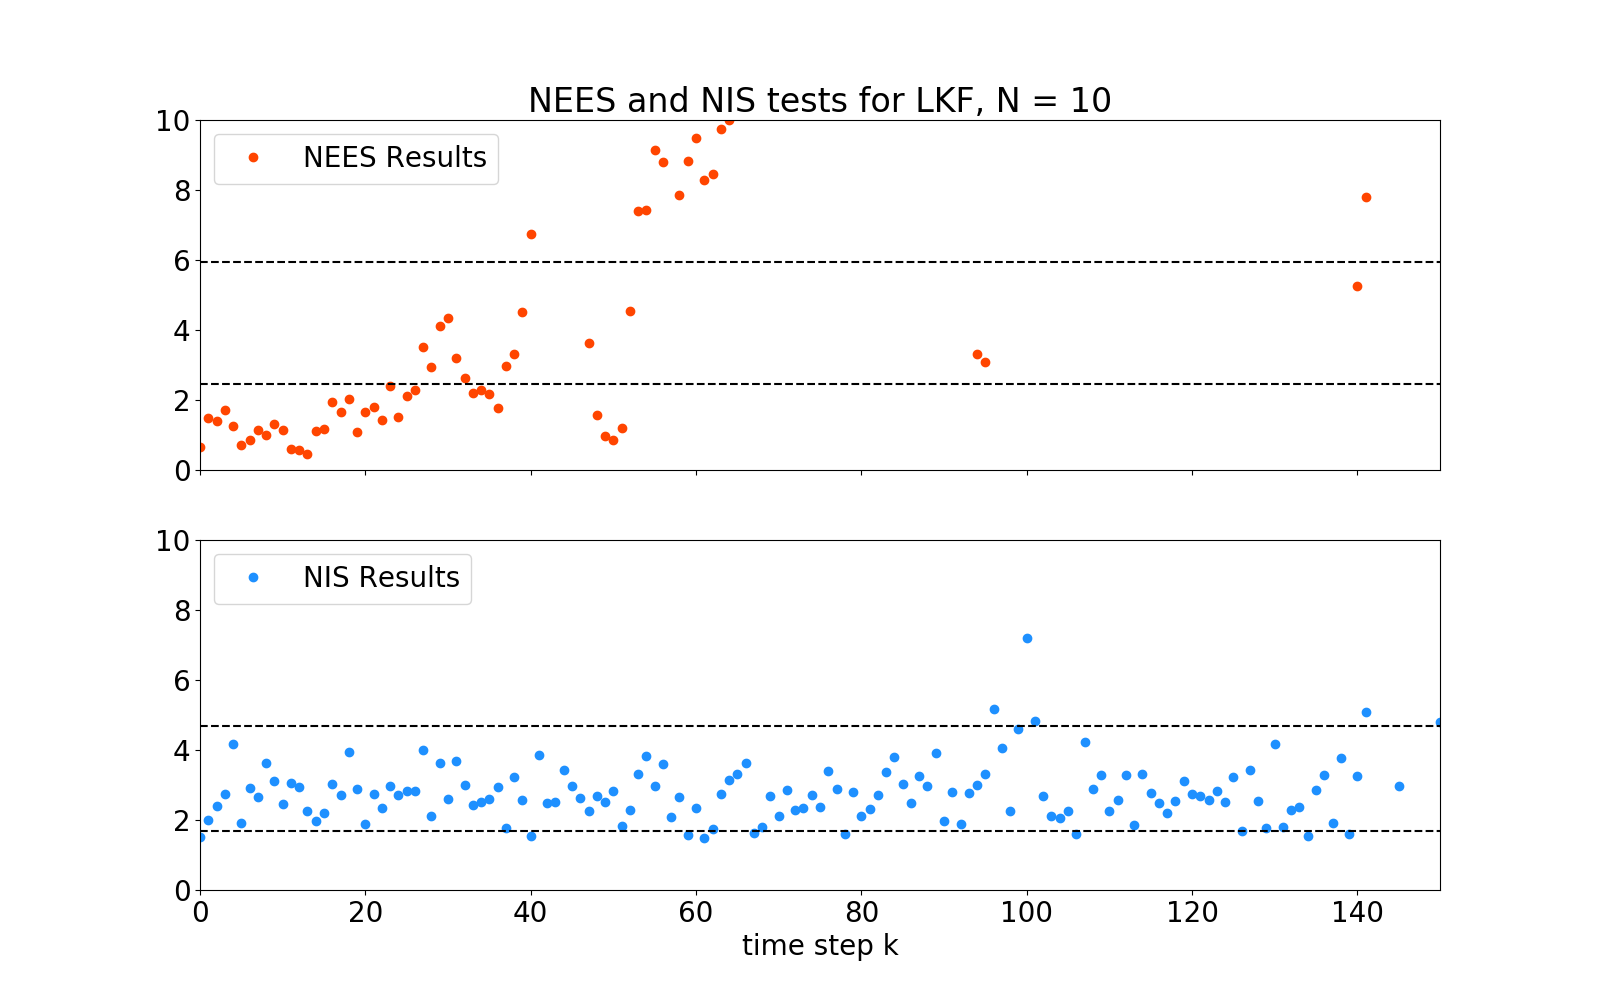
\includegraphics[width=\textwidth]{Figures/NEESNIS_lkf_N10Q1.0E-06.png}
	\caption{NEES and NIS chi-square results over time for N = 10 simulated trajectories. Guessed $Q_{KF} = 10^{-6} \cdot I_{2 x 2}$.}
	\label{fig:neesnis_lkf_Qbig}
\end{figure}

In the second iteration of the tuning process, the Kalman filter was initialized with an internal process noise of $Q_{KF} = 10^{-12} \cdot I_{2 x 2}$. 
The results of this test can be seen in Figure \ref{fig:neesnis_lkf_Qsmall}. 
In both tests---but especially the NEES---the values are biased above the upper confidence bound. 
This low bias lead to the conclusion that the guessed $Q_{KF}$ is too small, and should be increased for as to avoid being smug. 
\begin{figure}[H]
	\centering
	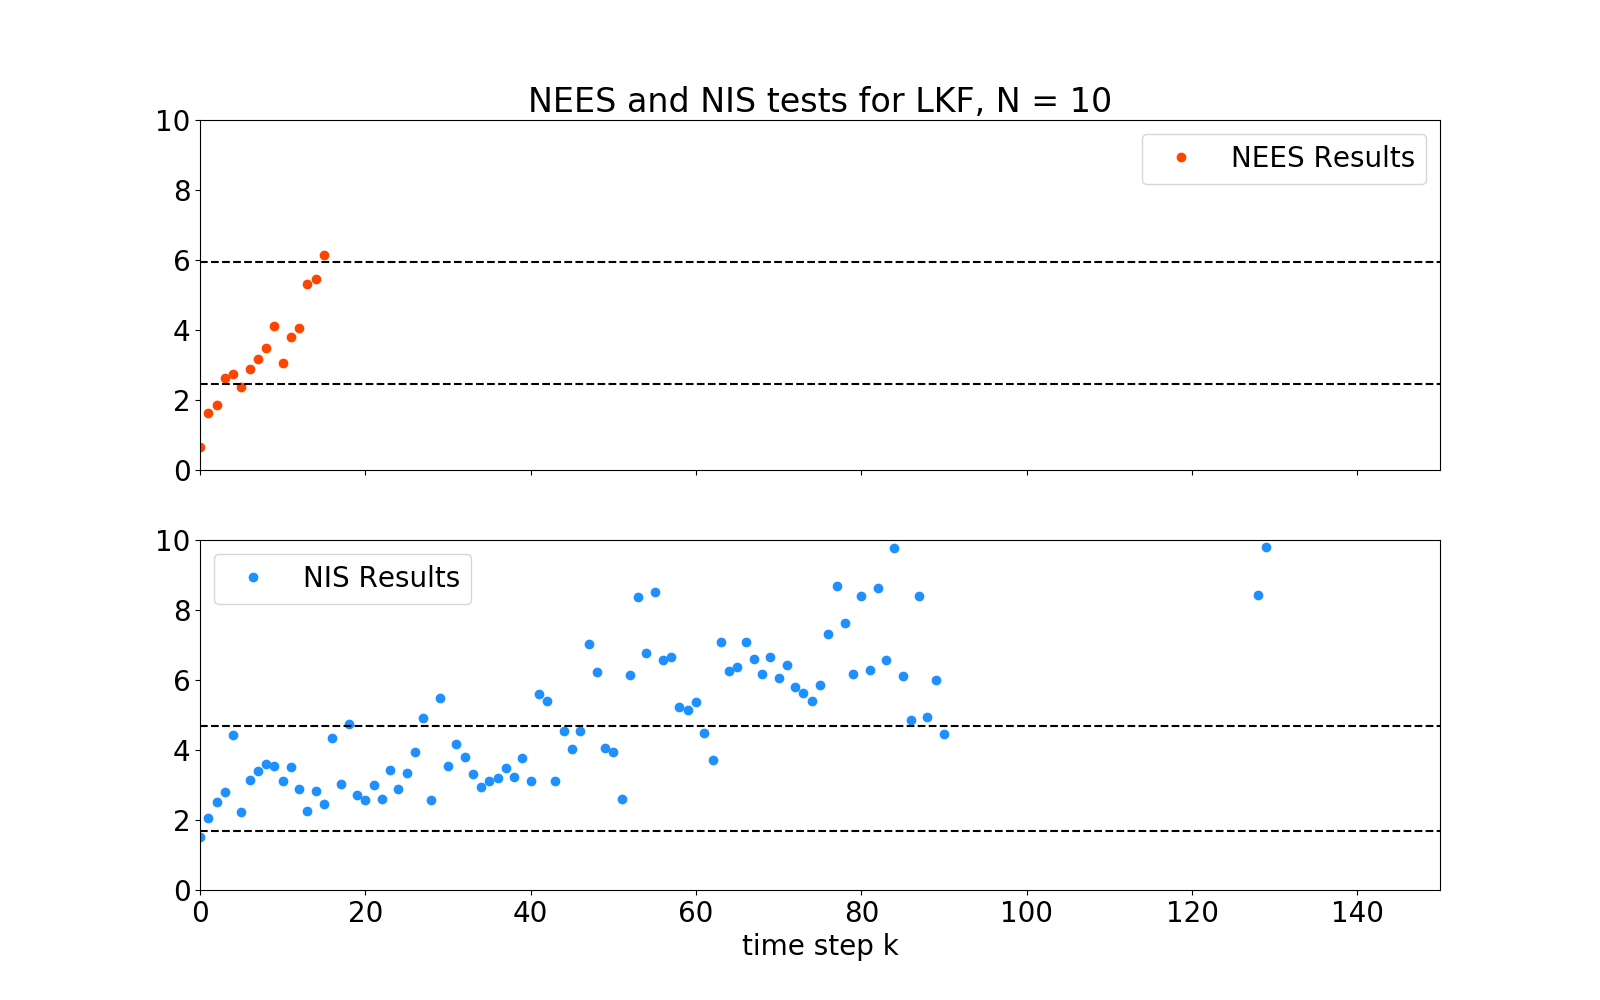
\includegraphics[width=\textwidth]{Figures/NEESNIS_lkf_N10Q1.0E-12.png}
	\caption{NEES and NIS chi-square results over time for N = 10 simulated trajectories. Guessed $Q_{KF} = 10^{-12} \cdot I_{2 x 2}$.}
	\label{fig:neesnis_lkf_Qsmall}
\end{figure}

In this third and final iteration of the tuning process, the Kalman filter was initialized with an internal process noise of $Q_{KF} = 10^{-9} \cdot I_{2 x 2}$. 
The results of this test can be seen in Figure \ref{fig:neesnis_lkf}.
While neither is perfect (due to the inherent ineptitude of the LKF to this orbit determination problem), the $Q_{KF}$ used here seems to be the best choice. 

\begin{figure}[H]
	\centering
	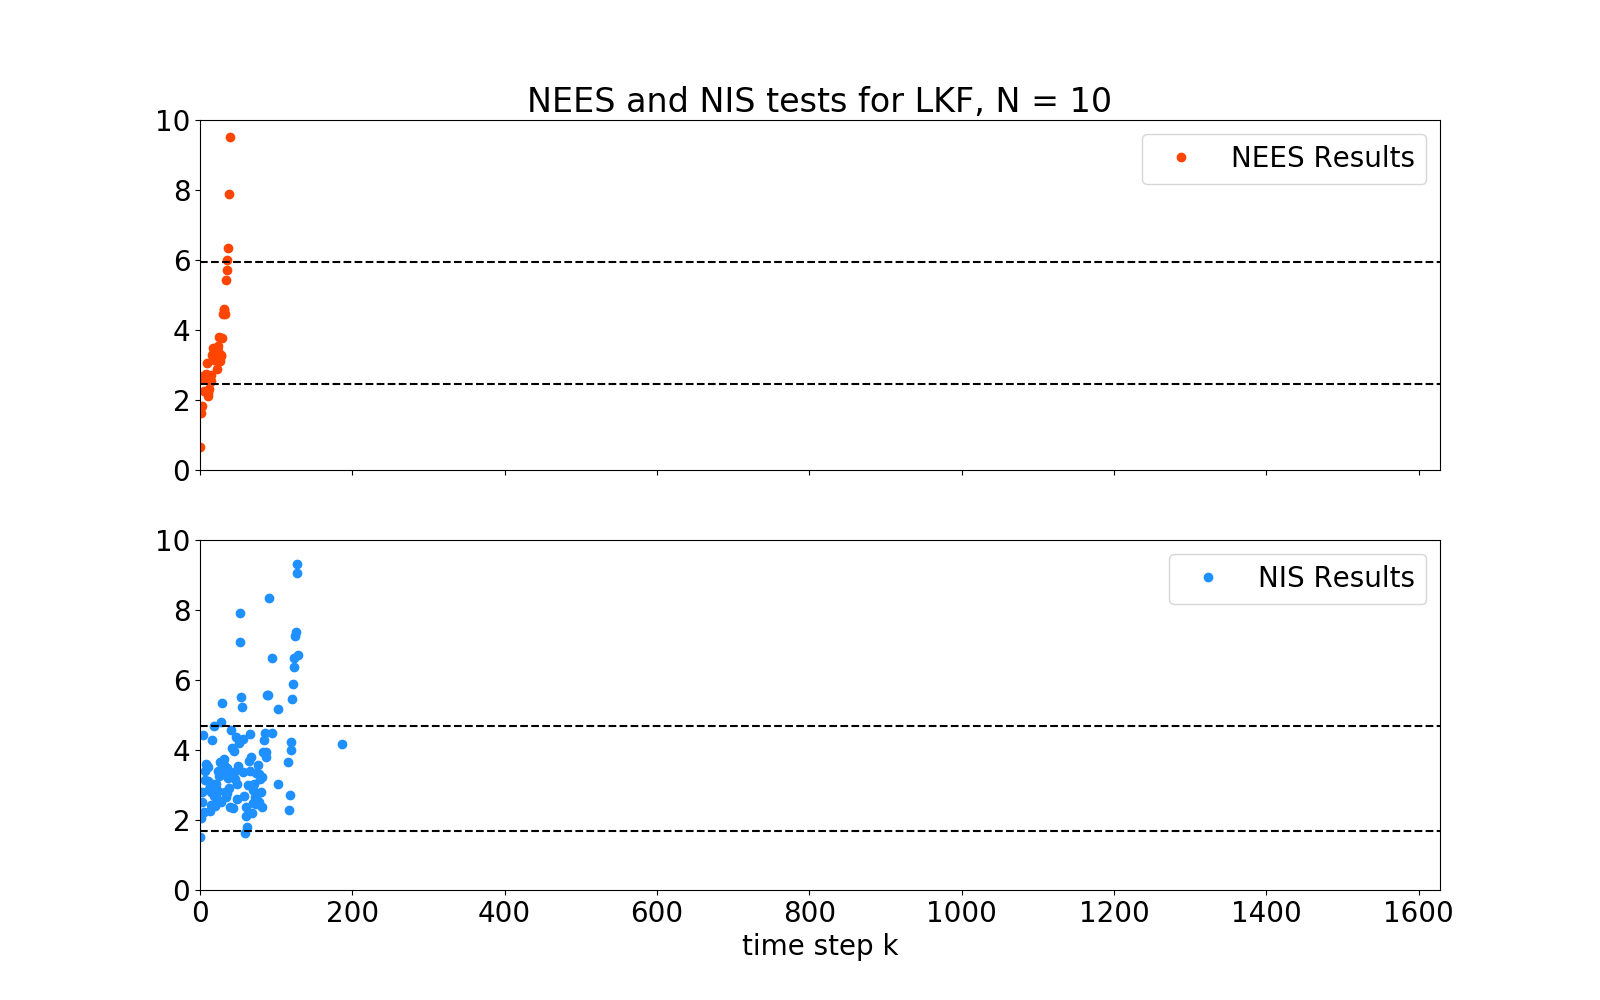
\includegraphics[width=\textwidth]{Figures/NEESNIS_lkf_N10Q1.0E-09.png}
	\caption{NEES and NIS chi-square results over time for N = 10 simulated trajectories. Guessed $Q_{KF} = 10^{-9} \cdot I_{2 x 2}$.}
	\label{fig:neesnis_lkf}
\end{figure}

\subsubsection{LKF Tuning Conclusions}
It should be noted that this process outlined above can be an automated process that begins by hopping between very large and very small guesses of $Q_{KF}$ and narrowing in until the ``best" performance is achieved. 
The specific definition of ``best" performance may be defined by the user of the program who is performing the tuning and does not necessarily represent an absolute optimization. 
However, since the LKF was shown to perform poorly for this orbit determination problem given this mild initial perturbation, much human intervention was required to assert the reliability of the results. 

Overall, as the findings findings in Section \ref{sec: Part I} indicated, the linearized dynamics used in the LFK become invalid as small initial perturbations eventually cause large deviations from the nominal trajectory. 
Figures \ref{fig:neesnis_lkf_Qbig} - \ref{fig:neesnis_lkf} corroborate these findings, and solidify our understanding of where the LKF is most capable: for small perturbations near the nominal trajectory.  

\subsubsection{Variable length measurements in NIS calculation}
The NEES and NIS confidence bounds are formed based on the number of random variables summed together. 
In general, this is equal to the number of states or measurements. 
Occasionally, multiple stations can observe the satellite at the same time.
This manifests as a single measurement with length $2p$.
As such, the number of random variables summed is $2p$, and the expectation of that sum should fall in a $2p$ (rather than p) degree of freedom $\mathcal{X}^2$ distribution. 
In order to generate comparable results for all time steps, when encountering a NIS value for a $2p$ measurement, the average NIS value of each individual measurement was calculated and used for analysis.


\subsection{The Extended Kalman Filter}
\label{sec: EKF}
The EKF relies less on linearizations about an initial nominal trajectory.
Instead of linearly propagating a deviation in a state, the EKF uses full nonlinear dynamics to propagate its full current state estimate. 
It then linearizes about its current estimate, rather than the initial nominal trajectory to perform time and measurement updates to the covariance.   
This allows the EKF to adjust for small perturbations from the nominal that may grow into large deviations with time, as it does not use the nominal trajectory for linearization. 

\subsubsection{EKF Typical Performance}
Figures \ref{fig:noisey_states} and \ref{fig:noisey_meas} show a typical noisy truth trajectory and accompanying noisey measurements as compared to the nominal, noiseless trajectory and measurements. 
Figure \ref{fig:ekf_est} shows a time history of a typical EKF estimate. 
The EKF, in contrast with the LKF, is much more capable of tracking the perturbed trajectory.  

\begin{figure}[H]
	\centering
	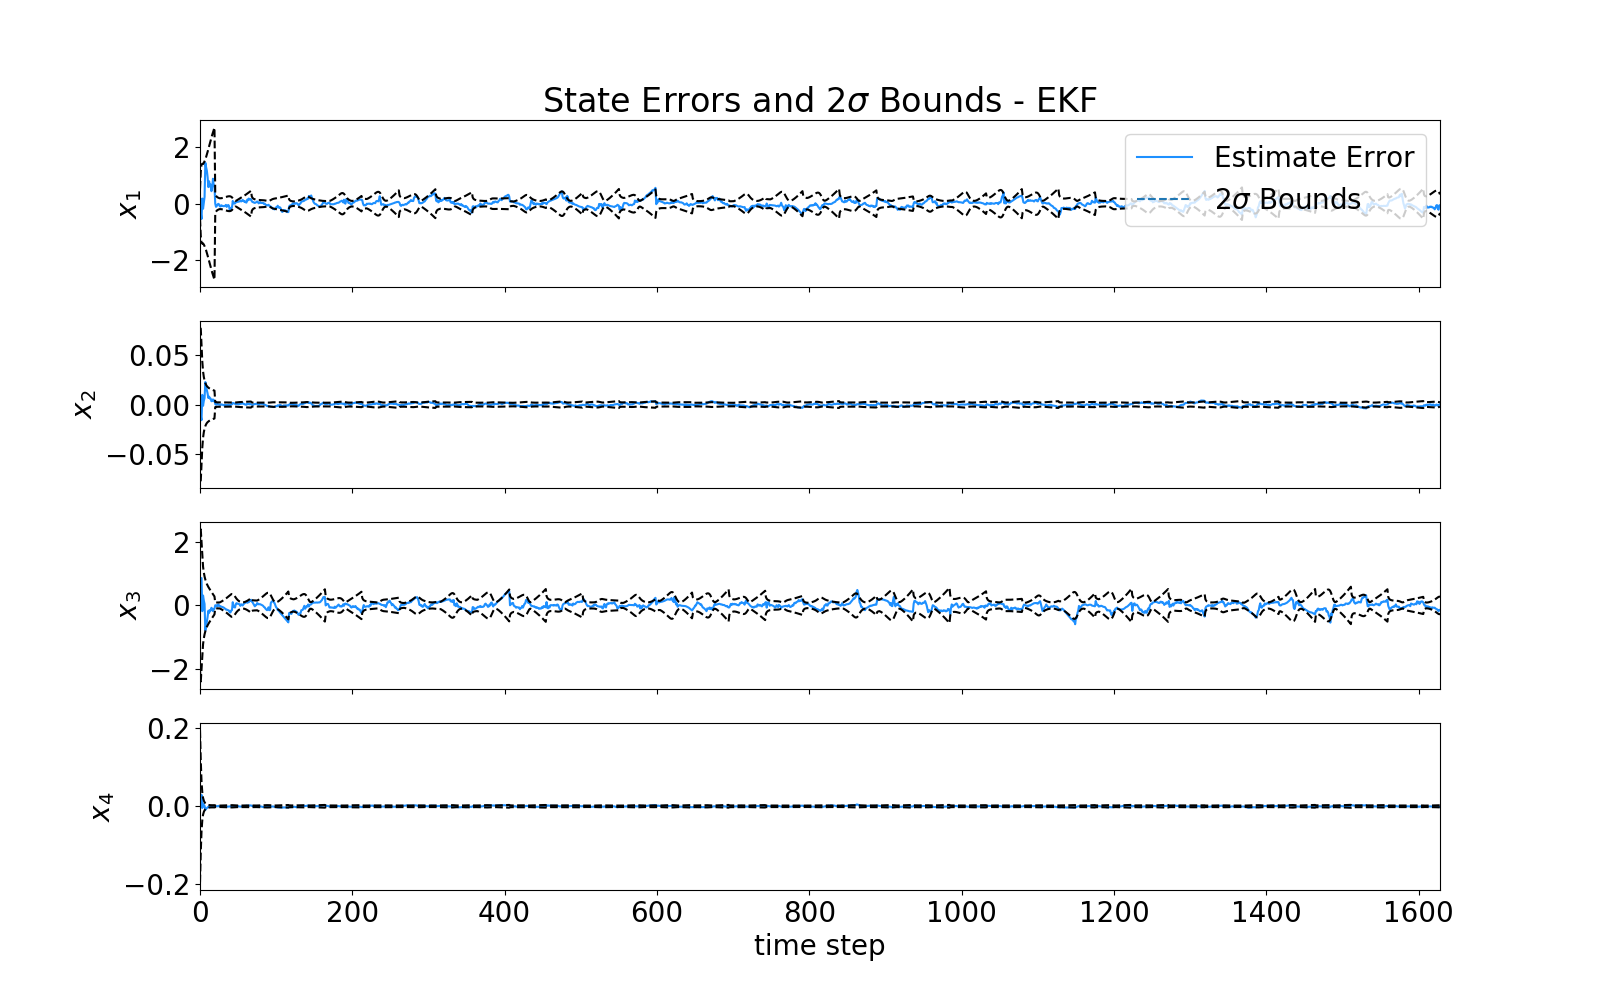
\includegraphics[width=\textwidth]{Figures/ekf_estimate_th.png}
	\caption{Typical EKF error estimate over the entire simulation period.}
	\label{fig:ekf_est}
\end{figure}


\subsubsection{NEES and NIS Tests}
Similar to before with the LKF, the EKF can be tuned by finding a $Q_{KF}$ that accurately models the actual process noise in the system. 
This is again done by starting with initial high and low magnitudes of $Q_{KF}$ and narrowing in based on the apparent bias n the NEES and NIS values. 
Note that, for all of the following tuning EKF operations, the results were generated using the same noisy trajectories and measurements as used before for the LKF. 

Figure \ref{fig:neesnis_ekf_Qbig} shows NEES and NIS results for the EKF when guessing a processes noise of $Q_{KF} = 10^{-6} \cdot I_{2 x 2}$. 
Note that it is apparent from this test that the guessed $Q_{KF}$ here is too big since the NEES and NIS values are both biased low in the confidence intervals. 
The filter in this case can be seen to be pessimistic, as it does not trust its estimate. 
\begin{figure}[H]
	\centering
	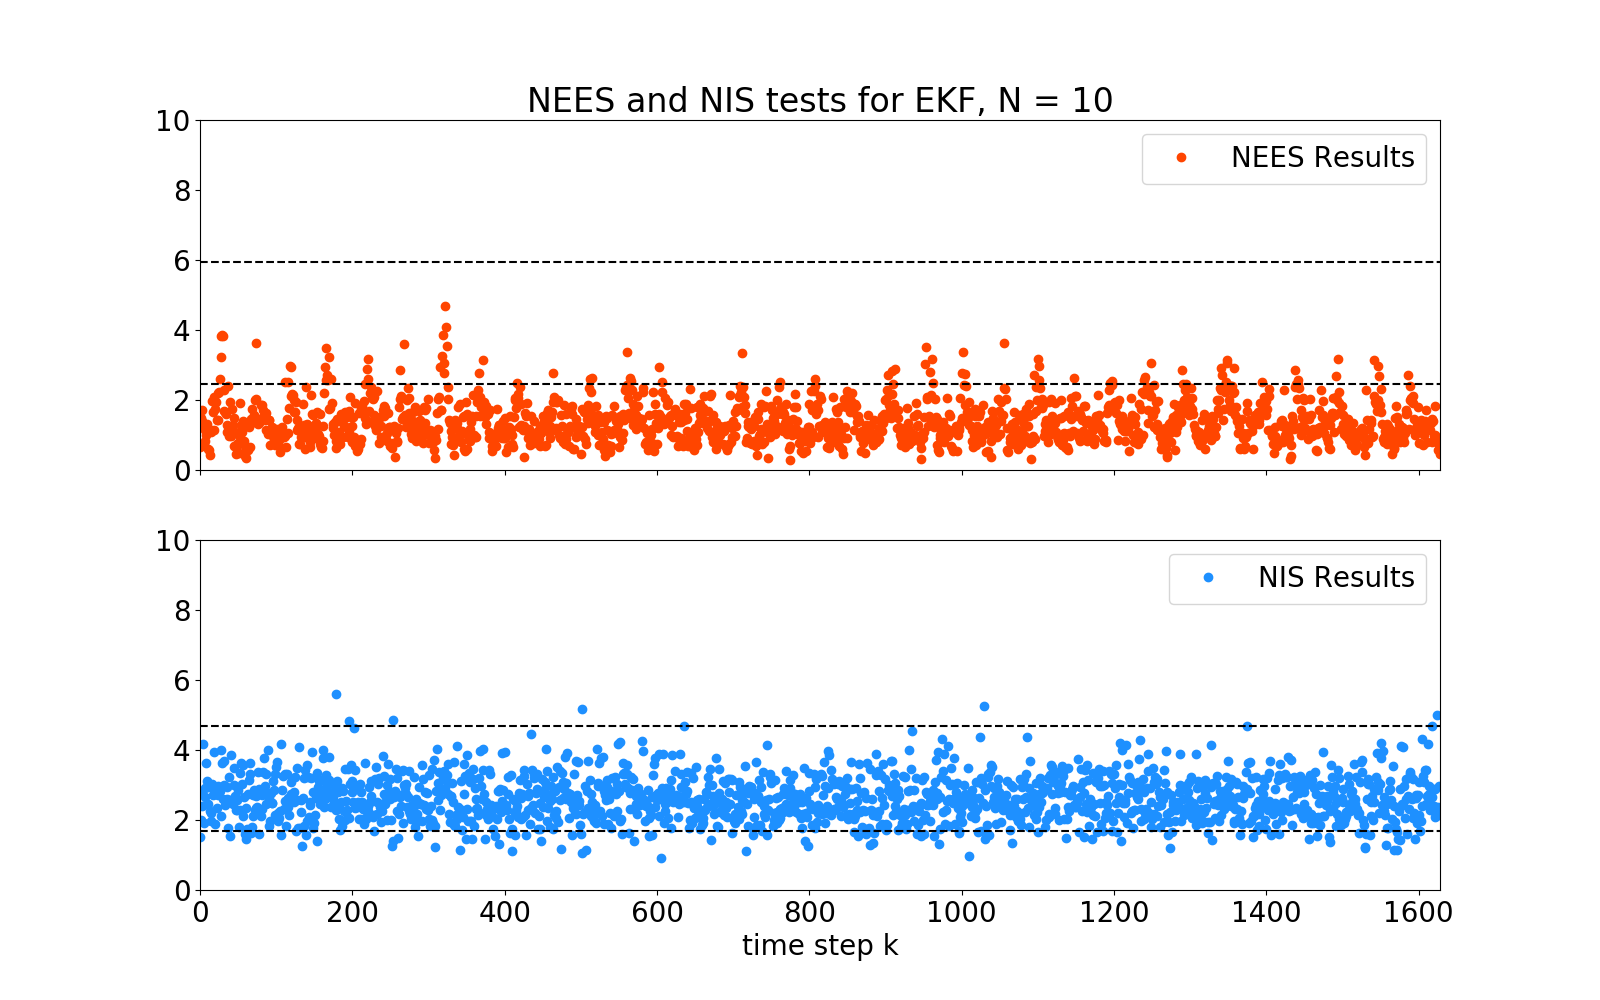
\includegraphics[width=\textwidth]{./Figures/NEESNIS_ekf_N10Q1.0E-06.png}
	\caption{NEES and NIS chi-square results over time for N = 10 simulated trajectories and $Q_{KF} = 10^{-6} \cdot I_{2 x 2}$.}
	\label{fig:neesnis_ekf_Qbig}
\end{figure}


Decreasing the guessed process noise to $Q_{KF}= 10^{-12} \cdot I_{2 x 2}$ yields the results seen in Figure \ref{fig:neesnis_ekf_Qsmall} in which the filter is smug. 
It is seen here trusting its estimate too much, and latching on to a trajectory that is not the truth data. 
\begin{figure}[H]
	\centering
	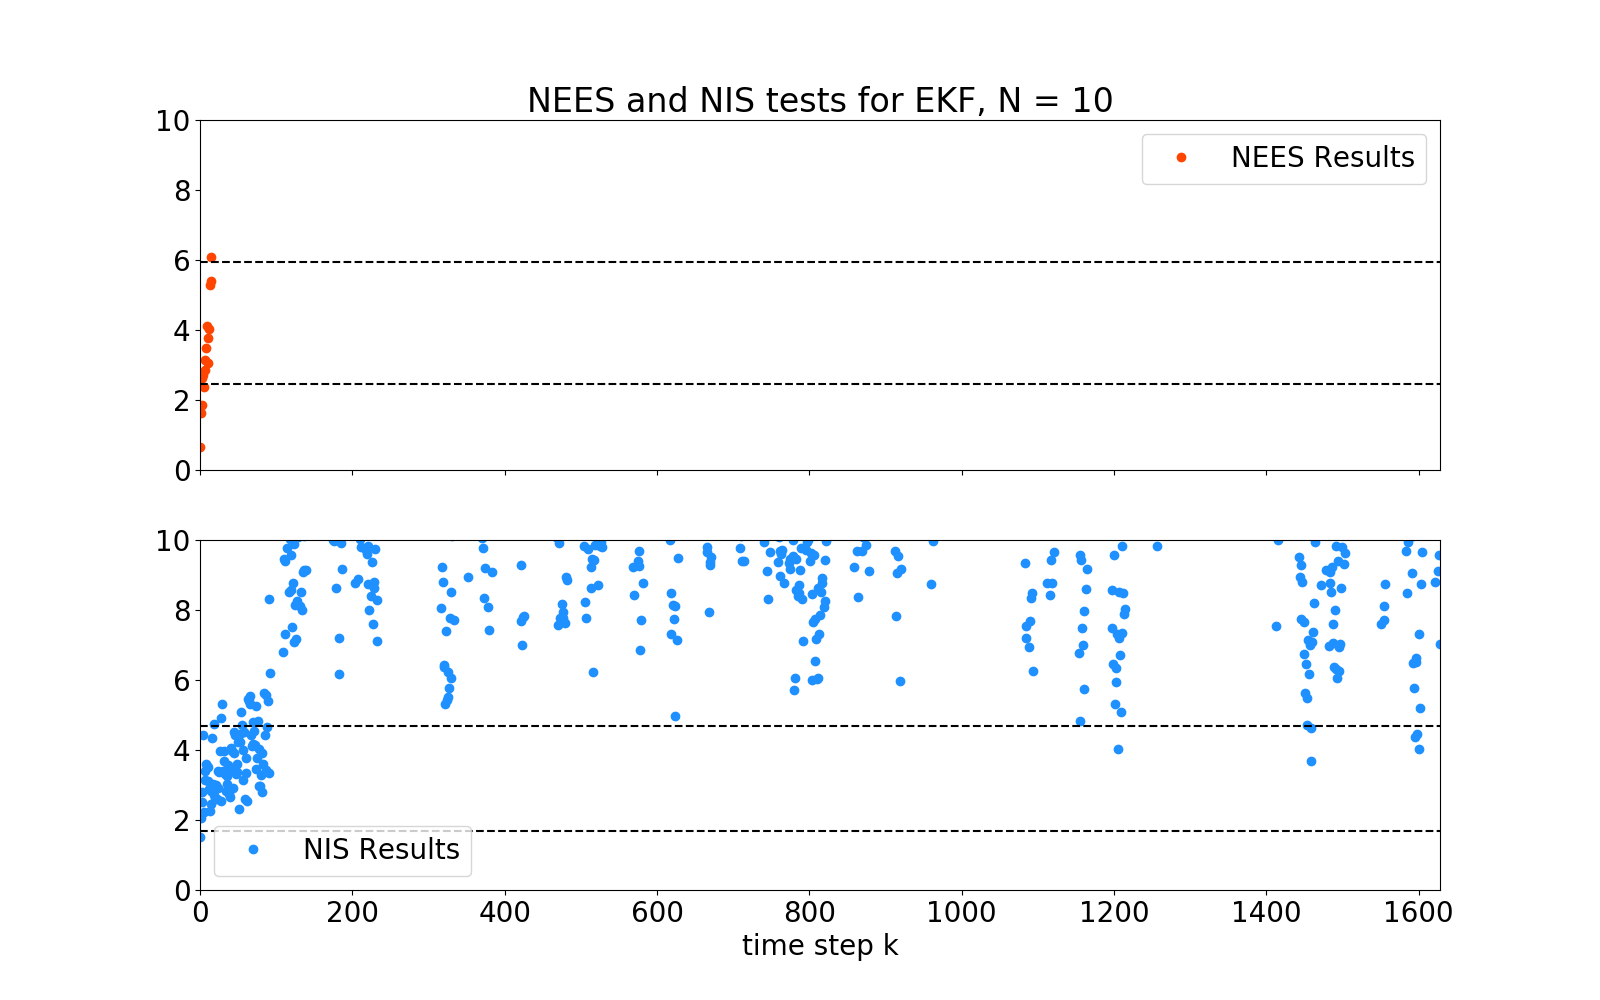
\includegraphics[width=\textwidth]{./Figures/NEESNIS_ekf_N10Q1.0E-12.png}
	\caption{NEES and NIS chi-square results over time for N = 10 simulated trajectories and $Q_{KF} = 10^{-12} \cdot I_{2 x 2}$.}
	\label{fig:neesnis_ekf_Qsmall}
\end{figure}

Here in Figure \ref{fig:neesnis_ekf}, the NEES and NIS results for the EKF are right spot on in terms of number of NEES and NIS values lying within the confidence bounds. 
This demonstrates a well-tuned filter. 
\begin{figure}[H]
	\centering
	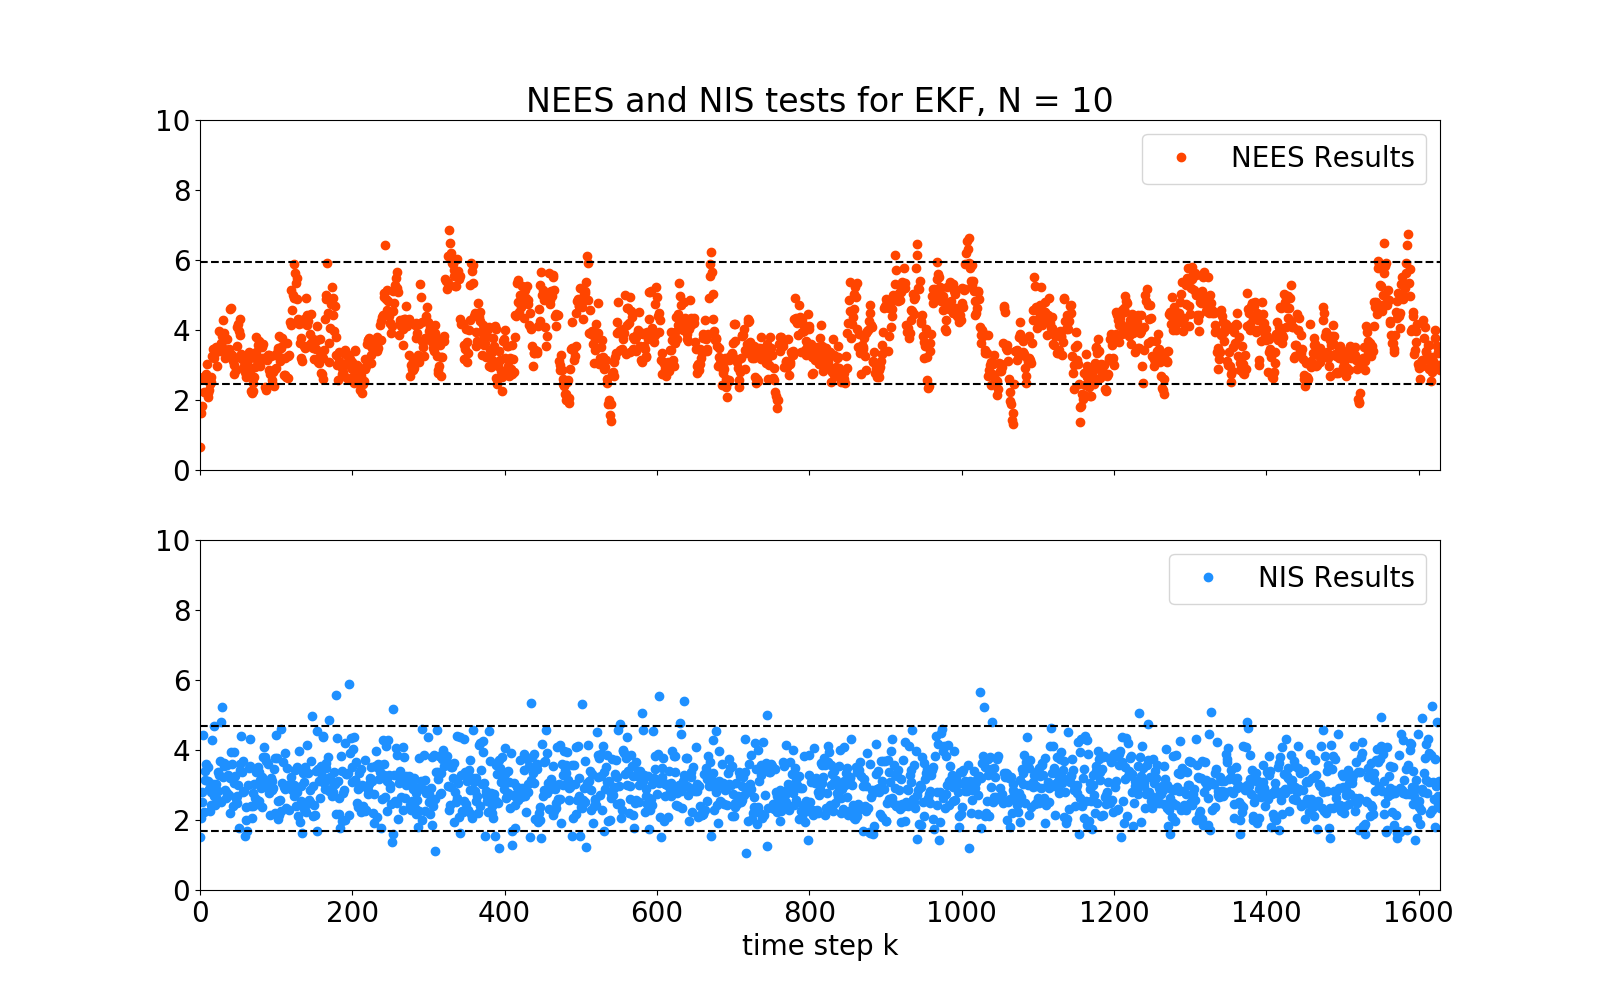
\includegraphics[width=\textwidth]{./Figures/NEESNIS_ekf_N10Q1.0E-09.png}
	\caption{NEES and NIS chi-square results over time for N = 10 simulated trajectories and $Q_{KF} = 10^{-9} \cdot I_{2 x 2}$.}
	\label{fig:neesnis_ekf}
\end{figure}

These results show the estimate tracking the truth trajectory more accurately for the duration of the simulations. 
Because the EKF continuously updates its internal 'nominal' trajectory, it's able to latch on to the perturbed trajectory and doesn't rely on stale information from the original nominal trajectory. 
This results in the filter's ability to keep up with the deviations from the original nominal trajectory, and estimate the truth trajectory accurately.


\section{Testing Without Ground Truth}
In addition to observing each filter's capabilities as compared to truth states and measurements, we estimated a trajectory from which only measurements were available. 
The results of these  are shown below for the LKF and EKF respectively using the tuned noise and covariance parameters. 
\begin{figure}[H]
	\centering
	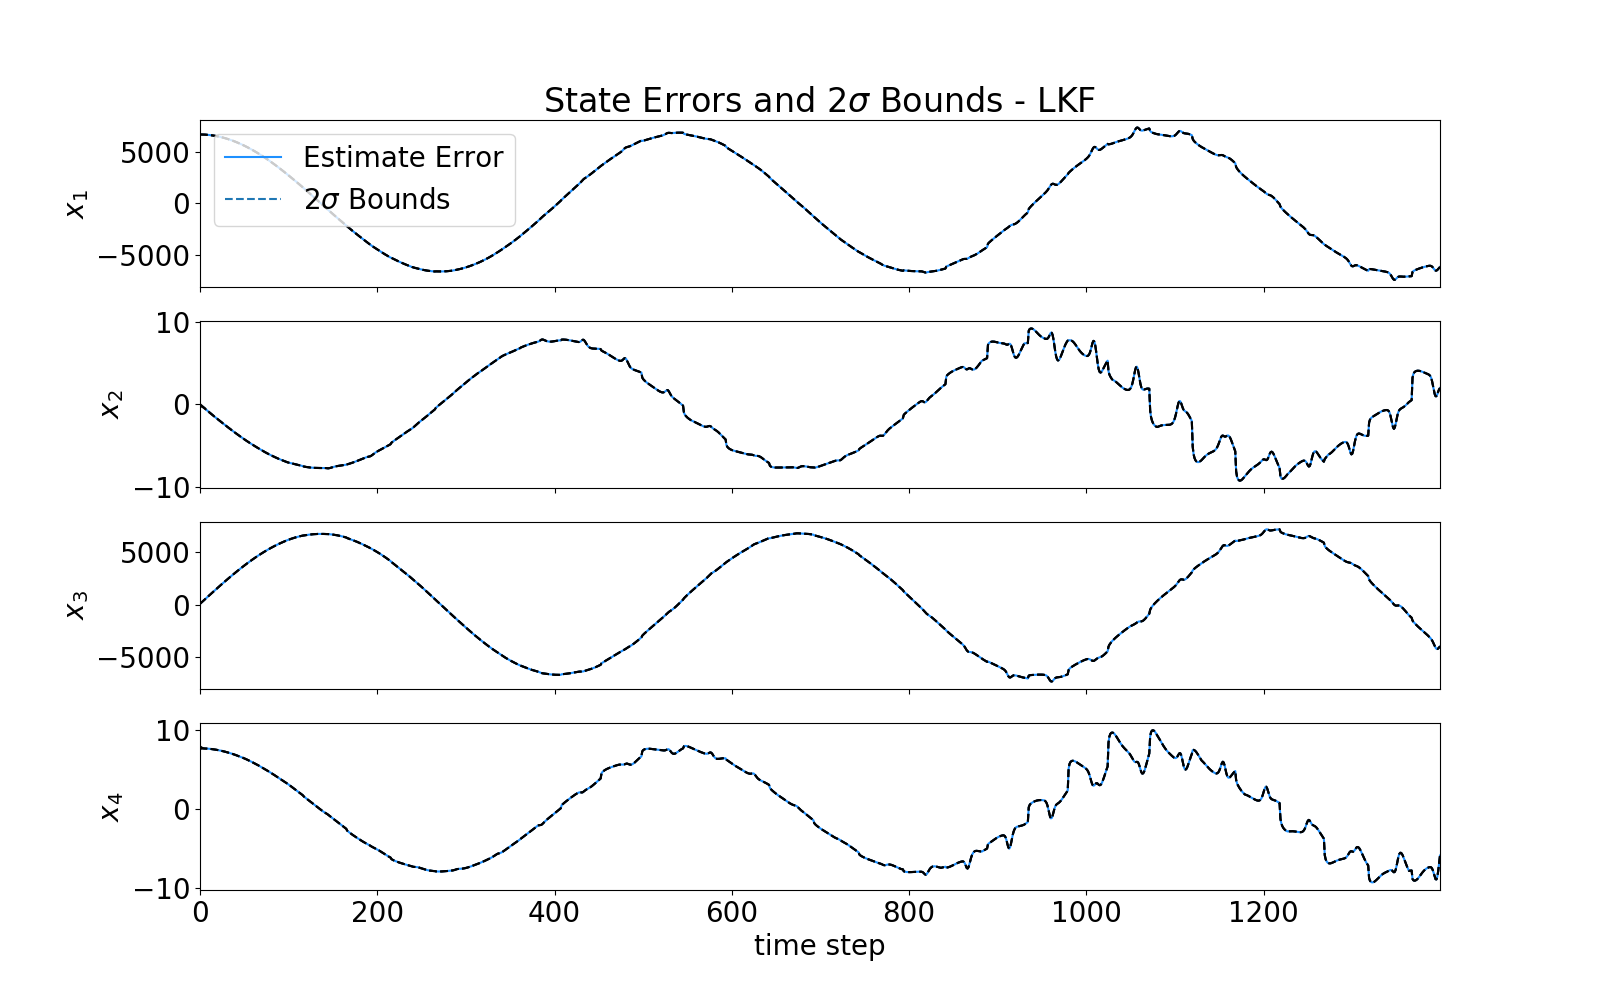
\includegraphics[width=\textwidth]{Figures/lkf_dataste_est.png}
	\caption{LKF results using assignment dataset.}
	\label{fig:lkf_dataset}
\end{figure}

\begin{figure}[H]
	\centering
	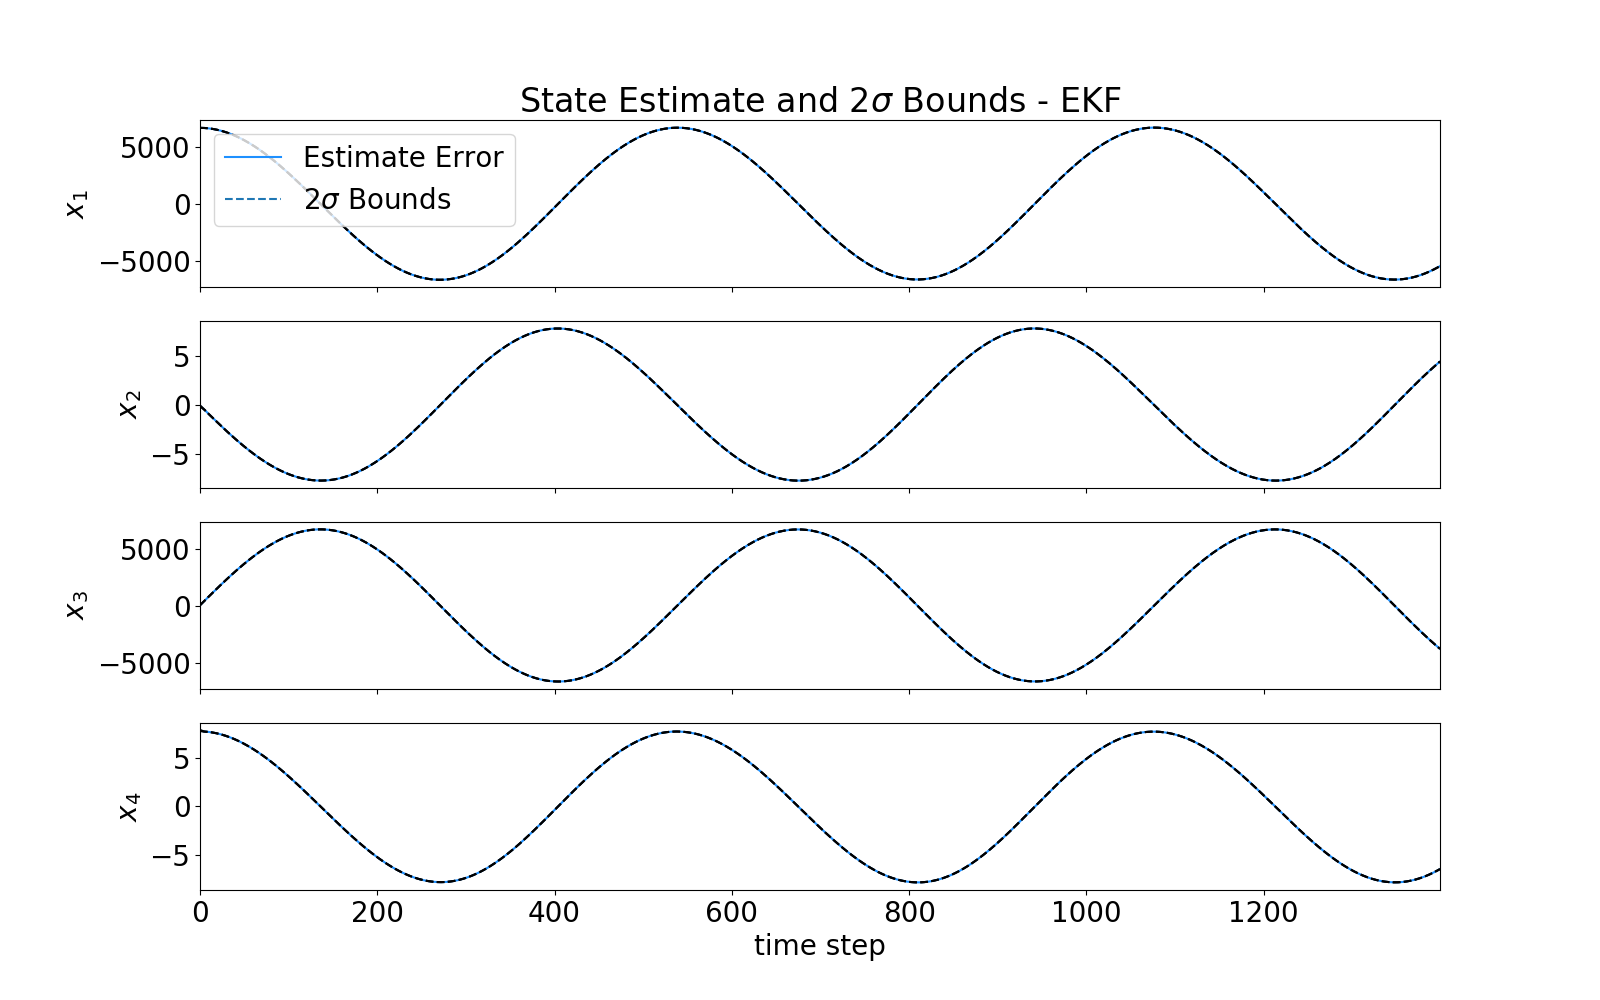
\includegraphics[width=\textwidth]{Figures/ekf_dataset_est.png}
	\caption{EKF results using assignment dataset.}
	\label{fig:ekf_dataset}
\end{figure}

The LKF estimate, begins with smooth, orbit-esque estimate and seems to track well for approximately 1/2 of an orbit. 
However, as time goes on, the estimate becomes less recognizable as an orbit trajectory - even though its covariance bounds shrink around the estimate 
From this observation, we can say that the LKF, as in other tests, is incapable of estimating the orbit after it has drifted a substantial distance from the nominal trajectory. 
The state deviation and error covariance are propagated based on jacobians evaluated on the nominal trajectory, so it's crucial that actual measurements originate near that nominal. 

The EKF seems to track the orbit adequately for the full duration of incoming measurements. 
This is because it's able to propagate its estimate with full nonlinear dynamics and linearize about its estimate, rather than a nominal trajectory, 
the EKF is able to keep up with the growing deviation from original nominal trajectory. 

We note that this data log contained some entries with no measurement data, indicating the spacecraft was not visible at that time by any station. 
For these measurements, in both the LKF and EKF, the filters skipped a measurement update, and performed multiple, single step, time updates until encountering another valid measurement.  

%%%%%%%%%%%%%%%%%%%%%%%%%%%%%%%%% CONCLUSION %%%%%%%%%%%%%%%%%%%%%%%%%%%%%%%%%
\section{Conclusion}
Through computational analysis, an implementation of both the Linearized Kalman Filter and Extended Kalman Filter were studied and tuned to better understand their capabilities. 
It was found, through trial and error, that increasing the process noise above what's actually included on the incoming data results in an unhealthy reliance on measurement data. 
Because a large process noise increases the error covariance with each time update, the error covariance grows too large for the filter to trust the dynamic system, and defaults to the measurements. 
If the filter believes underestimates the process noise, the filter becomes smug, and rejects incoming information from the measurements. 

We also note that the LKF is ill-equipped to handle orbit problems, or any problem where small initial deviations only increase with time.
In contrast, because the EKF can update the trajectory about which it linearizes with full nonlinear equations, it's able to keep up with the eventual large deviations seen in orbit problems.  

%%%%%%%%%%%%%%%%%%%%%%%%%%%%%%%%% APPENDIX %%%%%%%%%%%%%%%%%%%%%%%%%%%%%%%%%
\newpage

\section*{Advanced Questions}
\subsection{Bugs}
Crawling on our laptop screen \\
underneath our keyboard's keys \\
\texttt{clear all, close all, clc} \\
just end us now. Please, bugs, please. \\
 
\subsection{The Unscented Kalman Filter}
The Unscented Kalman Filter is a variant on the Kalman filter which makes still fewer linear approximations than the EKF. 
The UKF samples $2n+1$ sigma points from the current estimate probability distribution function (PDF) and uses these to perform time and measurement updates.
The sigma points are carefully selected to represent the current multivariate PDF. 
This allows for a more accurate propagation of estimate and covariance through time and measurement updates, as no linearized jacobians are evaluated. 
The results of an implementation the UKf on the data set used for previous tests are shown below.

\begin{figure}[H]
	\centering
	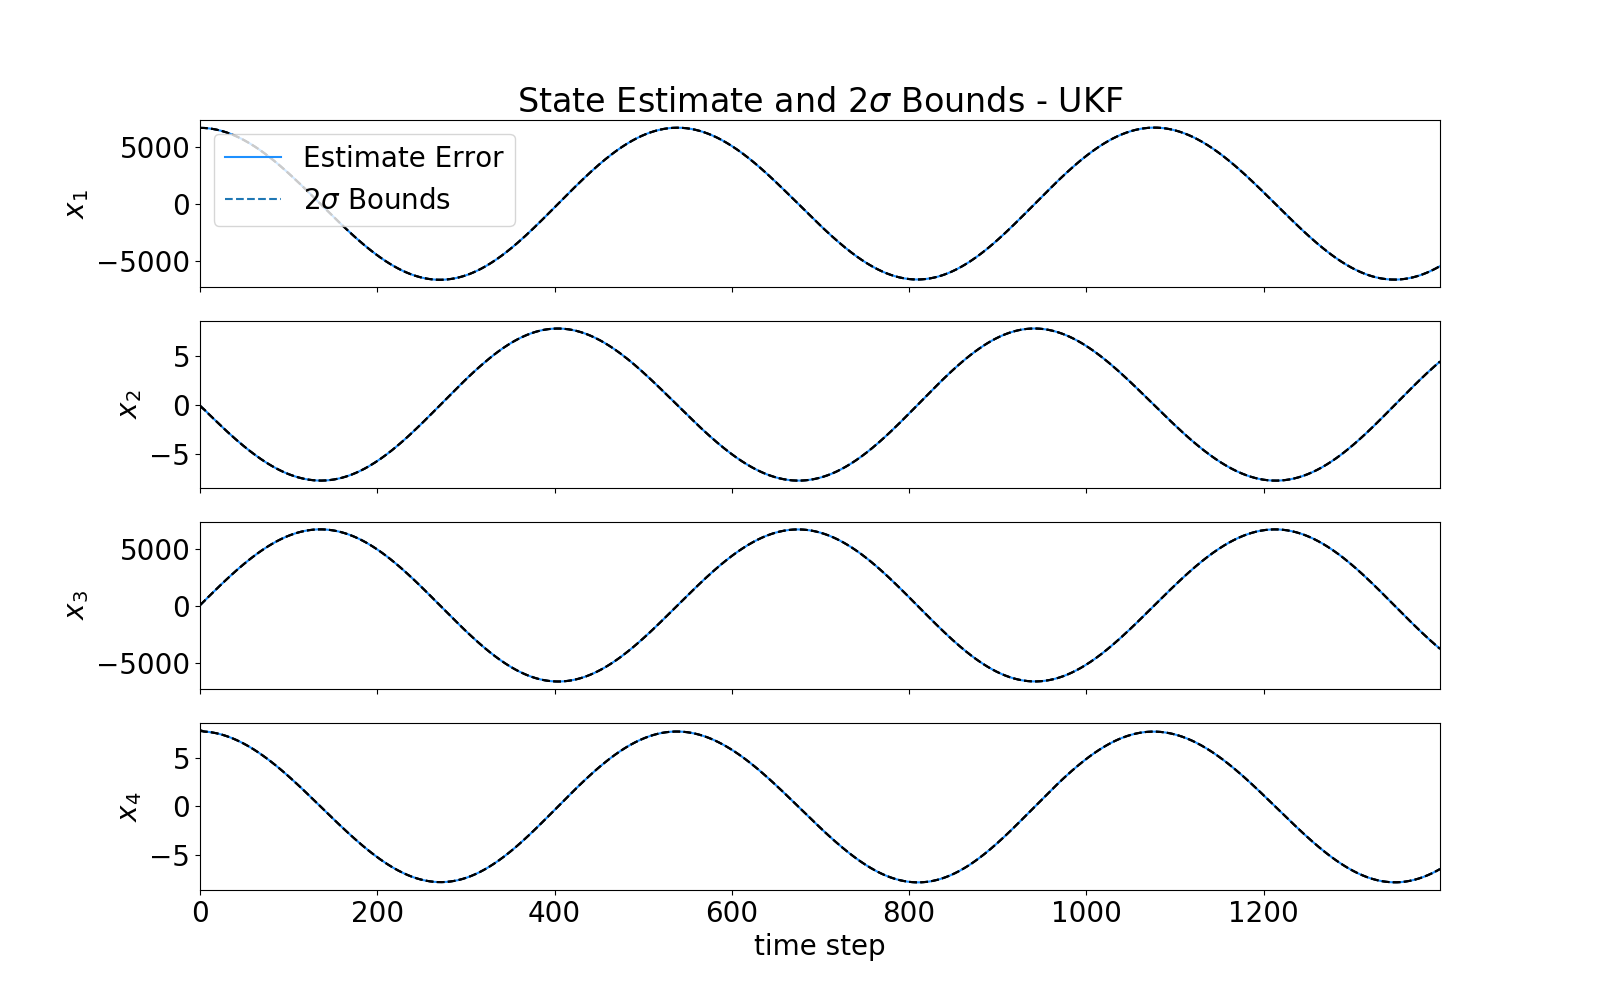
\includegraphics[width=\textwidth]{Figures/ukf_dataset_est.png}
	\caption{UKF results using assignment dataset.}
	\label{fig:ukf_dataset}
\end{figure}

The UKF was also tuned using NEES and NIS tests to validate the input parameters. 
Similarly to the LKF and EKF, the UKF is highly dependent on its knowledge of process noise in the system. 
The UKF has additional tuning parameters pertaining to the approximate pdf created from the sigma points. For this analysis, a Gaussian distribution was approximated, but higher-moment parameters of the pdf can be specified as well. 
It was found that, for this particular problem, changing the distance from the mean at which sigma points are sampled changes very little about the final estimate. 
This may indicate that, for the perturbations used, and the type of system used, the covariance remains mostly Gaussian even with the nonlinear transformations between time steps and in to measurement space.   


\begin{figure}[H]
	\centering
	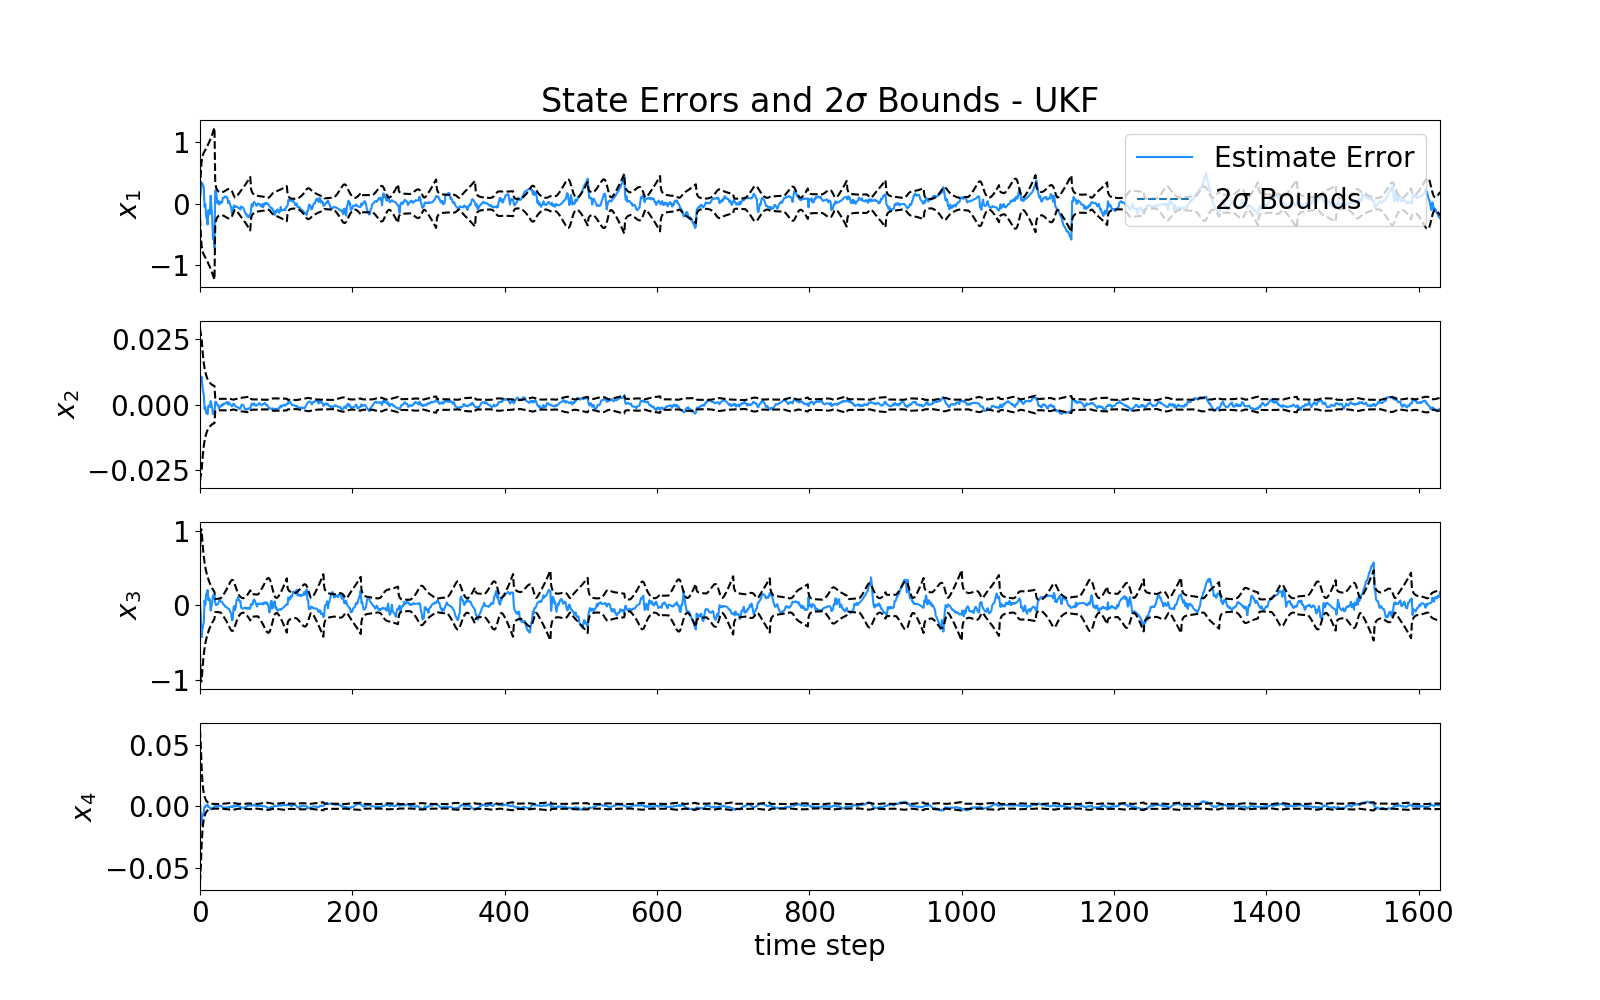
\includegraphics[width=\textwidth]{Figures/ukf_estimate_th.png}
	\caption{Typical UKF error estimate over the entire simulation period.}
	\label{fig:ukf_est}
\end{figure}

\begin{figure}[H]
	\centering
	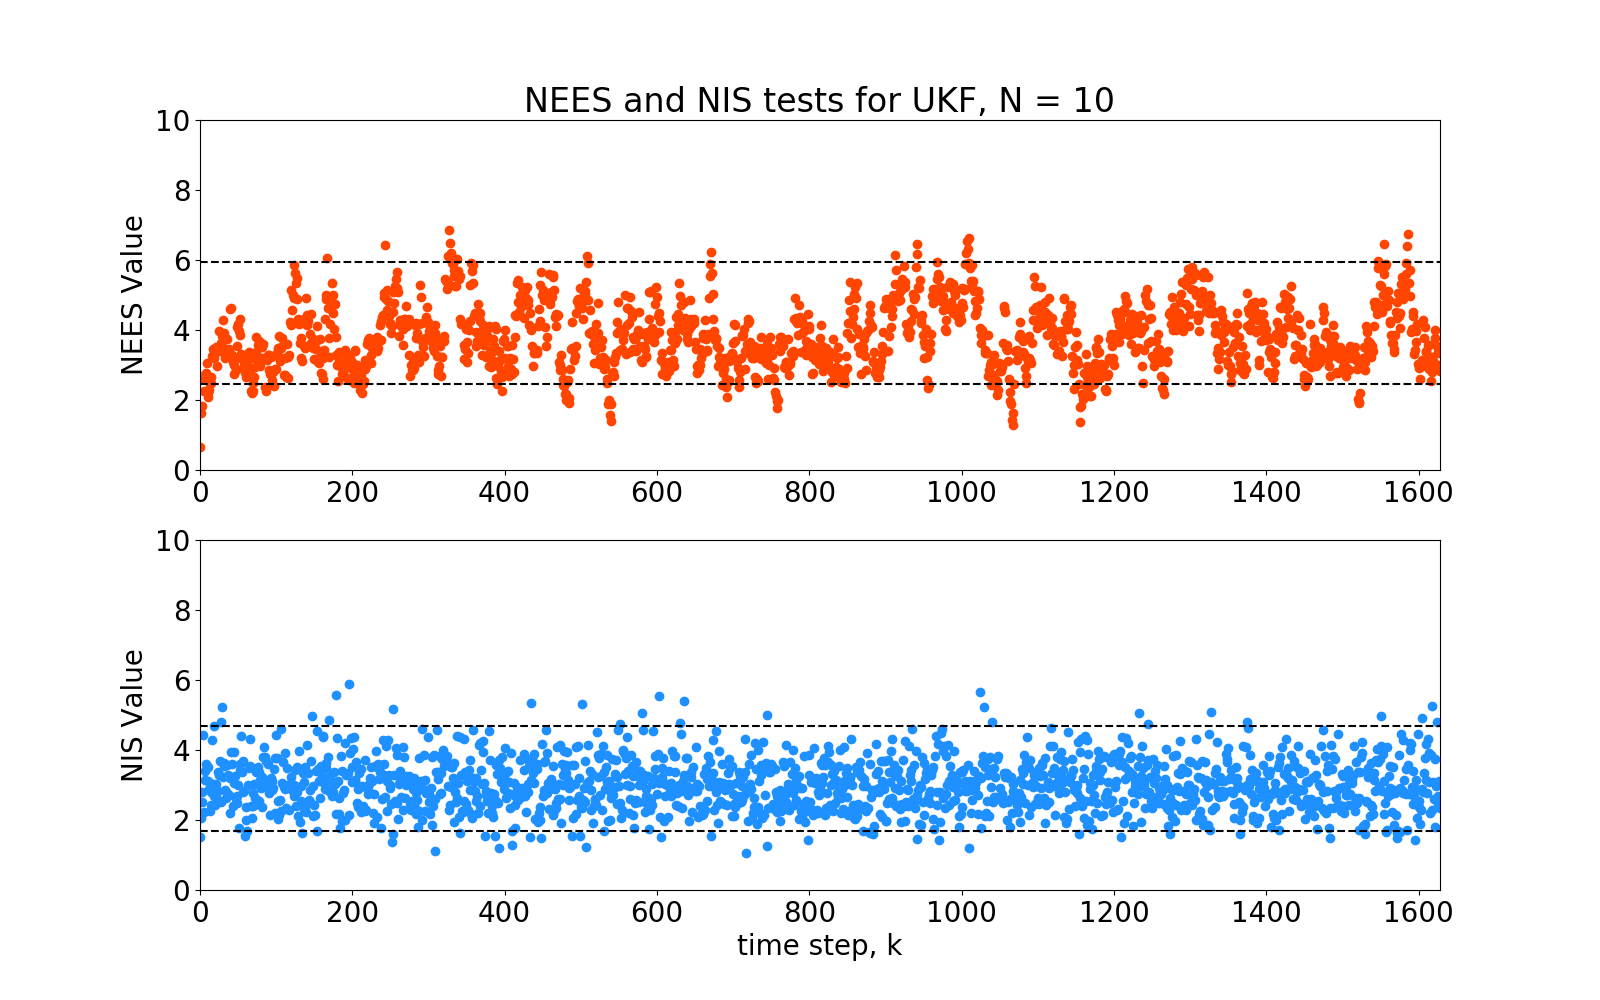
\includegraphics[width=\textwidth]{./Figures/NEESNIS_ukf_N10Q1.0E-09.png}
	\caption{NEES and NIS chi-square results over time for N = 10 simulated trajectories.}
	\label{fig:neesnis_ukf}
\end{figure}


\newpage
\section*{Appendix}
%\lstinputlisting{../main.m}
The code used to generate the data used in this study is written in python and can be found in the attached .zip file.
\vspace{5mm}
The general layout of the code is as follows:\\
The filters are written in an object-oriented structure, where each non-linear filter is an object that extends the abstract base class KF. 
They are written with a similar instantiation and usage as the scipy.integrate.ode class. 
The scripts labeled main\_* are used to run the use-cases of the LKF, EKF, and UKF. 
Note that the truth trajectory generation code is called once independently and saved to files as to avoid re-generating on each run.



\end{document}


